\documentclass[table,12pt]{book}
\usepackage[utf8]{inputenc}
\usepackage[english]{babel}
\usepackage{csquotes}
\usepackage{geometry}
\usepackage{tikz,lipsum,lmodern}
\usetikzlibrary{calc}
\usepackage[most]{tcolorbox}
\usepackage{listings}
\usepackage{xcolor}
\usepackage[hidelinks]{hyperref}
\usepackage{tikzpagenodes}
\usepackage{imakeidx}
\usepackage[style=authoryear,bibstyle=authoryear]{biblatex}
\usepackage{enumitem}
\setitemize{noitemsep,topsep=0pt,parsep=0pt,partopsep=0pt}
\usepackage{makeidx}
\usepackage[nottoc,numbib]{tocbibind}
\usepackage{tgtermes}
\usepackage[T1]{fontenc}

\def\checkmark{\tikz\fill[scale=0.4](0,.35) -- (.25,0) -- (1,.7) -- (.25,.15) -- cycle;} 

\addbibresource{ref.bib}

\makeindex

\input{set}
\input{cmd}
\newcommand{\abstractionDef}{\textbf{abstraction}: Representation that is purposely missing details to focus attention on purpose of the object / idea / etc. being represented.}

\newcommand{\acceptanceCriterionDef}{\textbf{acceptance criterion}: A statement about functionality that, when satisfied, mean the functionality has been satisfactorily implemented.}

\newcommand{\agileDef}{\textbf{Agile}: A software process model and philosophy for managing and developing software projects. Agile values: Individuals and interactions, working software, customer collaboration, and responding to change.}

\newcommand{\attitudeTowardRiskCsfDef}{\textbf{attitude toward risk CSF}\index{attitude toward risk (cognitive style facet)}: How willing a person is to take chances in software (risk-tolerant vs. risk-averse)}

\newcommand{\businessCapabilityDef}{\textbf{business capability}: ``the potential of a business resource (or groups of resources) to produce customer value by acting on their environment via a process using other tangible and intangible resources'' \parencite{Michell2011AFA}}

\newcommand{\classDiagramDef}{\textbf{class diagram}: Visualization of how classes are built in relation to other classes in object-oriented software. Includes properties and methods of individual classes and ``has a'' and ``is a'' relationships between classes.}

\newcommand{\clientDef}{\textbf{client}\index{client}\index{customer} (a.k.a. customer): One or more people or organizations who are requesting the software be made and have decision-making authority about the software (e.g., because they are paying for it or otherwise providing resources).}

\newcommand{\clientServerArchitectureDef}{\textbf{client-server architecture}: Overall code design characterized by one component (the server) responding to requests and providing resources while other components (clients) request those resources.}

\newcommand{\codeDecayDef}{\textbf{code decay} (AKA software rot): Reduction of code quality over time. Can result in decreased maintainability, more bugs, and irretrievable failure.}

\newcommand{\codeSmellDef}{\textbf{code smell}: Aspect of code that indicates the code is of poor quality (e.g., has detriments to read- ability and maintainability).}

\newcommand{\cognitiveStyleFacetsDef}{\textbf{cognitive style facets (CSFs)\index{cognitive style facets}}: Five aspects of users that affect how they solve problems in software: Motivations\index{motivations (cognitive style facet)}, information processing style\index{information processing style (cognitive style facet)}, computer self-efficacy\index{computer self-efficacy (cognitive style facet)}, attitude toward risk\index{attitude toward risk (cognitive style facet)}, learning style\index{learning style (cognitive style facet)}}

\newcommand{\cognitiveStyleFacetValueDef}{\textbf{cognitive style facet value (A.K.A., cognitive style)}: A position on the spectrum of a cognitive style facet}

\newcommand{\cognitiveStyleHeuristicsDef}{\textbf{Cognitive Style Heuristics (CSH)\index{cognitive style heuristics}}: Eight principles of interaction design\index{interaction design} for finding and fixing usability\index{usability} bugs in software. They are based around different cognitive styles\index{cognitive styles} different people use when they problem-solve in software.}

\newcommand{\cognitiveStylePersonasDef}{\textbf{cognitive style personas}: Three specialized personas (Abi, Pat, and Tim) used for making software UI designs more usable to people with different cognitive styles.}

\newcommand{\cognitiveWalkthroughDef}{\textbf{cognitive walkthrough\index{cognitive walkthrough}}: A usability inspection method that involves stepping through a user interface as a user, stopping to ask specific questions about the user's experience \parencite{nielsen94}.}
\newcommand{\componentDef}{\textbf{component}: Within a codebase, a unit of the code containing related functionality. Ideally, is both replaceable and reusable.}

\newcommand{\computerSelfEfficacyCsfDef}{\textbf{computer self-efficacy CSF\index{computer self-efficacy (cognitive style facet)}}: A person's confidence in their ability to use computers or software (low vs. high)}

\newcommand{\contingencyDef}{\textbf{contingency}: A future event or circumstance that may occur but depends on known and unknown factors. Can be difficult to predict far ahead of time.}

\newcommand{\couplingDef}{\textbf{coupling}: The degree to which one unit of code is dependent on another.}

\newcommand{\dodDef}{\textbf{Definition of Done (DoD)}: The set of acceptance criteria which, once satisfied, mean a user story has been satisfactorily implemented.}

\newcommand{\eisenhowerMatrixDef}{\textbf{Eisenhower matrix}: 2x2 grid for helping decide whether to do, delegate, schedule, or eliminate a task based on its urgency and importance.}

\newcommand{\encapsulationDef}{\textbf{encapsulation}: In object-oriented programming, (1) combining data and the methods that act upon that data into one unit of code or (2) preventing external direct access to data within a unit of code.}

\newcommand{\estimationDef}{\textbf{estimation}: Figuring out ahead of time how long a task is likely to take.}

\newcommand{\eventualConsistencyDef}{\textbf{eventual consistency}: Characteristic of software systems where different parts of the system can have less up-to-date information (e.g., state, data) than other parts but the inconsistencies are temporary.}

\newcommand{\extensibleDef}{\textbf{extensible}: Built in such a way to support adding more functionality later.}

\newcommand{\extremeProgrammingDef}{\textbf{Extreme Programming (XP)}: Agile framework that prioritizing customer satisfaction and communication, short development cycles, iteration, frequent releases, code review, teamwork, pair programming, required unit testing, and only implementing functionality that's needed.}

\newcommand{\fistOfFiveDef}{\textbf{fist of five}: A method for gauging and building group consensus that uses a 6-level voting system (zero to five fingers).}

\newcommand{\focusGroupDef}{\textbf{focus group} (in usability engineering): A moderated discussion between researcher and a small number of potential users (usually 6-12) during which the researcher tries to gather information about the participants' attitudes, opinions, motivations, concerns, and problems related to a specific product or topic.\parencite{odimegwu00}}

\newcommand{\functionalRequirementDef}{\textbf{functional requirement}: Description of what functionality the software needs to have.}

\newcommand{\ganttChartDef}{\textbf{Gantt chart}: Horizontal bar chart showing start and end times of activities within a project schedule, along a timeline.}

\newcommand{\genderMagMethodDef}{\textbf{GenderMag Method:} A method for finding and fixing gender-inclusivity bugs in software that uses a specialized cognitive walkthrough and the customizable Abi, Pat, and Tim personas \parencite{burnett16}}

\newcommand{\guiDef}{\textbf{graphical user interface (GUI)}: A user interface with interactive graphics, in contrast to a text-based user interface.}

\newcommand{\groundRulesDef}{\textbf{ground rules}: A set of statements about the team, agreed to by each team member, for avoiding team conflict and dysfunction.}

\newcommand{\heuristicEvaluationDef}{\textbf{heuristic evaluation}: A usability inspection method where evaluators independently check that a design reflects a set of heuristics, then compare results \parencite{nielsen90}.}

\newcommand{\highFidelityPrototypeDef}{\textbf{high-fidelity prototype}: A polished illustration that looks like a finished, publishable user interface design (especially a GUI). Almost always digital.}

\newcommand{\highLevelArchitectureDef}{\textbf{high-level architecture}: Abstract representation of overall code design; covers all parts of the software.}

\newcommand{\ideDef}{\textbf{IDE}: Integrated development environment. Software specifically for creating software.}

\newcommand{\idealDaysDef}{\textbf{ideal days}: The number of days it would take to complete the work if the work could be 100\% focused on.}

\newcommand{\inclusiveSoftwareDesignDef}{\textbf{inclusive software design}: A type of software user interface design with the goal of increasing usability for traditionally under-served user populations while also increasing usability for mainstream users.}

\newcommand{\incrementDef}{\textbf{increment}: In software, a measurable increase in functionality.}

\newcommand{\informationProcessingStyleCsfDef}{\textbf{information processing style CSF\index{information processing style (cognitive style facet)}}: How a person looks through or absorbs information in software (comprehensively vs. selectively)}

\newcommand{\interactionDesignDef}{\textbf{interaction design}: An approach to technology design that involves helping users understand what's happening with the technology, what just happened, and what they can do \parencite{norman13}.}

\newcommand{\interactionDiagramDef}{\textbf{interaction diagram}: Visualization of collaboration between different parts of software.}

\newcommand{\investDef}{\textbf{INVEST}: Characteristics of good user stories (independent, negotiable, valuable, estimable, small, testable) \parencite{wake}.}

\newcommand{\iterationDef}{\textbf{iteration}: Verb: Revision. Noun (in Agile): A time-boxed software development cycle.}

\newcommand{\iterationPlanDef}{\textbf{iteration plan}: In Agile, establishing what will be done during a development cycle.}

\newcommand{\learningStyleCsfDef}{\textbf{learning style CSF}: How a person prefers to move through software (tinkering vs. by process)}

\newcommand{\lowFidelityPrototypeDef}{\textbf{low-fidelity prototype}: A \textbf{rough} sketch of a user interface design (especially a GUI). Can be hand-drawn or digital.}

\newcommand{\maintenanceDef}{\textbf{maintenance}: Development activities that improve software but that are unrelated to implementing new features (e.g., correcting bugs, improving organization of code, etc.).}

\newcommand{\msmDef}{\textbf{managerial skill mix (MSM)}: Three categories of skills used by managers: (1) interpersonal, (2) technical, (3) administrative/conceptual.}

\newcommand{\mediumFidelityPrototypeDef}{\textbf{medium-fidelity prototype}: A careful and detailed illustration of a user interface design (especially a GUI). Can be hand-drawn, but digital is more common.}

\newcommand{\methodDef}{\textbf{method}: A pre-established way of achieving a specific outcome.}

\newcommand{\microservicesArchitectureDef}{\textbf{microservices architecture}: Overall code design characterized by multiple independent components that each run in their own process and communicate between one another without direct access.}

\newcommand{\mitigationPlanDef}{\textbf{mitigation plan}: What you will do if a contingency happens.}

\newcommand{\monolithArchitectureDef}{\textbf{monolith architecture}: Overall code design characterized by being in one or few pieces; cannot be easily divided into components that run separately and are independently useful.}

\newcommand{\motivationCsfDef}{\textbf{motivation CSF}: Why someone is using the software (task completion vs. interest)}

\newcommand{\mvpDef}{\textbf{minimum viable product (MVP)}: A low-effort or low-expense effort that results in you being able to better estimate whether people will want to use your product---before the product is fully developed.\parencite{olsen15}}

\newcommand{\nonFunctionalRequirementDef}{\textbf{non-functional requirement}: Description of how well software is expected to perform.}

\newcommand{\paperPrototypeDef}{\textbf{paper prototype}: A hand-drawn sketch used to communicate a potential user interface design to be implemented, especially a graphical user interface design \parencite{snyder03}.}

\newcommand{\personaDef}{\textbf{persona}\index{persona}: A fictional character that represents a subset of users in a target audience. Personas are used in marketing and UI design to help with focusing on particular groups of users and customers \parencite{pruitt10,martin12}.}

\newcommand{\planningPokerDef}{\textbf{planning poker}: In Agile, a consensus-based method of assigning estimates to a task that involves individuals on a team each making their own estimate privately, then sharing with the team, discussing, and re-estimating as needed.}

\newcommand{\productBacklogDef}{\textbf{Product Backlog}: In Agile Scrum, an ordered list of all that is known to be needed to improve a product.}

\newcommand{\projectManagementDef}{\textbf{project management}: The process of planning and executing a project while balancing the time, cost, and scope constraints.}

\newcommand{\projectManagementSystemDef}{\textbf{project management system}: Software for planning, organizing, and otherwise carrying out a project.}

\newcommand{\projectNetworkDef}{\textbf{project network}: Graph showing the order in which a project's activities are to be completed.}

\newcommand{\projectPriorityMatrixDef}{\textbf{project priority matrix:} 3x3 grid for documenting how to respond when there are potential changes to a project's time, cost, or scope. Options: Only positive change allowed (constrain), negative change allowed (accept), or positive change sought (enhance).}

\newcommand{\qualityAttributeDef}{\textbf{quality attribute}: A characteristic of software used to describe how good it is.}

\newcommand{\raciMatrixDef}{\textbf{RACI matrix}: In project management, a chart for defining which roles are responsible (R) and accountable (A) for a task or deliverable and which roles should be consulted (C) or informed (I) about the status of the task or deliverable.}

\newcommand{\refactoringDef}{\textbf{refactoring}: Improving code design without changing what the code does.}

\newcommand{\releasePlanDef}{\textbf{release plan}: What will be completed for a specific software release and when the release will occur.}

\newcommand{\requirementDef}{\textbf{requirement}: A rule the software must conform to: What the software must do, how well it must do what it does, or the software's limitations or constraints.}

\newcommand{\requirementsElicitationDef}{\textbf{requirements elicitation}: The process of gathering requirements from project stakeholders.}

\newcommand{\requirementsSpecificationDef}{\textbf{requirements specification}: Converting stakeholder requests into written requirements.}

\newcommand{\riskDef}{\textbf{risk}: Estimated probability of a negative contingency given known and unknown factors.}

\newcommand{\sequenceDiagramDef}{\textbf{sequence diagram}: Interaction diagram showing how different participants (e.g., users, software components, classes, etc.) collaborate during a single use case.}

\newcommand{\serviceDef}{\textbf{service}: A unit of software that received and fulfills requests.}

\newcommand{\schedulingDef}{\textbf{scheduling}: Deciding when project activities are to be completed, how long they will take, and what resources are needed to complete them.}

\newcommand{\scrumDef}{\textbf{Scrum}: An Agile framework ``for developing and sustaining complex products.'' \parencite{schwaber2020scrum}}

\newcommand{\sdlcDef}{\textbf{software development lifecycle (SDLC)}: Phases through which a software's development proceeds: requirements, design, implementation, testing, maintenance.}

\newcommand{\softwareArchitectureDef}{\textbf{software architecture}: Code design. Can be shown at different levels of abstraction and detail.}

\newcommand{\softwareEngineeringDef}{\textbf{software engineering}: The art and science of using different methods to efficiently create extensible, sustainable programs that solve problems people care about.}

\newcommand{\softwareProcessModelDef}{\textbf{software process model}: A philosophy and/or set of approaches for software development and/or software project management.}

\newcommand{\spikeDef}{\textbf{spike}: A quick and to-the-point investigation for gathering information to help the team answer a question or choose a development path.}

\newcommand{\sprintBacklogDef}{\textbf{Sprint Backlog}: In Scrum, the set of activities to be completed during a Sprint (from Product Backlog), the associated Sprint Goal, and a plan for completing the activities.}

\newcommand{\srsDef}{\textbf{Software Requirements Specification (SRS)}: A document that contains software requirements.}

\newcommand{\stakeholderDef}{\textbf{stakeholder}: Anyone who is or will be affected by the software or its development (e.g., clients, companies, users, developers, managers, politicians, etc.)}

\newcommand{\storyPointsDef}{\textbf{story points}: A method for estimating an activity based on its size relative to other activities. Scale established by team.}

\newcommand{\sustainabilityDef}{\textbf{sustainability}: Degree to which software can continue to function over time (e.g., measured in time and how well the software is functioning).}

\newcommand{\taskManagementSystemDef}{\textbf{task management system}: Software for planning and organizing project activities.}

\newcommand{\technicalDebtDef}{\textbf{technical debt}: Time and resources you (or someone else) will need to spend on modifying your software in the future because of the poor decisions you're making in the present.}

\newcommand{\techStackDef}{\textbf{tech stack}: The set of programming languages, frameworks, and other technologies chosen or needed for implementing a piece of software.}

\newcommand{\thinkAloudProtocolDef}{\textbf{think-aloud protocol}: A method for gathering feedback about the usability of a design that involves a test user speaking their thoughts as they interact with the design \parencite{lewis93}. More information: \url{https://tinyurl.com/think-aloud-protocol}}

\newcommand{\tripleConstraintDef}{\textbf{triple constraint}: In project management, the three limiting factors that govern project execution: time, cost, and scope. Scope includes quality. Cost includes spending money and resources.}

\newcommand{\tuckmanDef}{\textbf{Tuckman's model of team development}: A five-stage model of how a team develops over time: (1) forming, (2) storming, (3) norming, (4) performing, (5) adjourning.}

\newcommand{\uatDef}{\textbf{user acceptance testing (UAT)}: Formally testing software with end-users to check not only whether it performs as expected but also whether end-users will use it. Typically performed before the software is released.}

\newcommand{\umlDef}{\textbf{UML}: Unified modeling language: A set of notation and methods for describing and designing software.}

\newcommand{\usabilityTestingDef}{\textbf{usability testing}: Observing people while they try to use your software.\parencite{barnum20}}

\newcommand{\userInterfaceDef}{\textbf{user interface (UI)}: What a user interacts with to operate a system (e.g., a graphical user interface, a command-line interface, a virtual or augmented reality interface, etc.).}

\newcommand{\useCaseDef}{\textbf{use case}\index{use case}: ``A contract for the behavior of the system under discussion'' \parencite{cockburn01}}

\newcommand{\userStoryDef}{\textbf{user story}: ``Short, simple descriptions of a feature told from the perspective of the person who desires the new capability, usually a user or customer of the system.'' \parencite{cohn}}

\newcommand{\validationDef}{\textbf{validation}: Confirming that software meets users' needs (``did we build the right software?'').}

\newcommand{\velocityDef}{\textbf{velocity}: In Agile, a measure of how much work is being completed.}

\newcommand{\verificationDef}{\textbf{verification}: Confirming that software satisfied its requirements (``did we build the software right?'').}

\newcommand{\waterfallDef}{\textbf{waterfall} (software process model): Way of going about software development and management that is characterized by extensive planning, comprehensive documentation, and moving linearly through stages of the software development lifecycle (SDLC).}
\input{col}
\input{sty}

\title{\Huge{Handbook of Software Engineering Methods}}
\author{Lara Letaw}
\date{\today}
 
\begin{document}
\nomargins
\begin{tikzpicture}[overlay,remember picture] 
\node[anchor=south] at ([yshift=-1.05in,xshift=0in]current page text area.south){\includegraphics[width=8.5in]{cover}}; 
\end{tikzpicture}

\maketitle

\tableofcontents

\yesmargins

\chapter{Introduction}

\begin{tikzpicture}[overlay,remember picture] 
\node[anchor=south] at ([yshift=5in,xshift=0.6in]current page text area.south){\includegraphics[width=10in]{intro}}; 
\end{tikzpicture} 

I won't tell you how to be a software engineer; You'll learn that over time by doing it. Instead, this book is about \textbf{software engineering methods}: Ways people achieve specific objectives in software engineering---that can save your project. My hope is that, after reading this book (or parts of it), you'll feel better equipped for software engineering.

\section{What's software engineering?}

Let's build a definition from the bottom up:\\

\begin{itemize}
\item Software engineering\index{software engineering} is \textbf{not} the same as \textbf{programming}
\item Software engineering involves trying to apply \textbf{methods}
\item Software engineering involves trying to make programs that have a long lifespan (\textbf{sustainable}\index{sustainability})
\item Software engineering involves trying to make programs that can be added to\marginpar{\methodDef\margindivider}\marginpar{\sustainabilityDef\margindivider}\marginpar{\extensibleDef\margindivider}\marginpar{\tripleConstraintDef\margindivider}\marginpar{\softwareEngineeringDef} (\textbf{extensible}\index{extensibility})
\item Software engineering involves trying to balance time, cost, and scope (the \textbf{triple constraint}\index{triple constraint})
\item Software engineering often involves \textbf{teamwork}\index{teamwork}
\item Software engineering involves trying to solve \textbf{problems people care about}
\item Software engineering involves both \textbf{artistry} and \textbf{science}.
\end{itemize}

\spacer
\textbf{Our definition:}

\begin{quote}
\textbf{Software engineering} is the art and science of using different methods to efficiently create extensible, sustainable programs that solve problems people care about.
\end{quote}

\section{What's the philosophy behind this book?}

My beliefs about software engineering influenced how I wrote this book. Some of my strongest beliefs about software engineering are described below.

\subsection{Software engineering is not black and white}
Throughout the book, I've tried to communicate that \textbf{software engineering is the gray area of computer science}. ``Right'' answers can be difficult to find and may not be reproducible in different contexts. Software engineering as a field also \textbf{keeps changing} as research scientists gather new findings, engineers develop new technologies, visionaries define new methods, and the outside world changes (e.g., a pandemic happened while I was writing this book and that changed how software engineering teams collaborate). Whereas in programming you might ask, ``Is this algorithm correct?'', questions in software engineering are more like, ``How does my team know this software is ready to release?'' or, ``People keep misinterpreting my code, how do I shift it toward better understandability\index{understandability} and maintainability\index{maintainability}?''

\subsection{Studying every detail of software engineering is a waste of time}\marginpar{\agileDef\margindivider}\marginpar{\softwareProcessModelDef\margindivider}\marginpar{\iterationDef\margindivider}\marginpar{\incrementDef}
I'm \textbf{not going to tell you everything} you need to know about software engineering because (1) what you need to know can be drastically different depending on \textbf{context} and (2) if I tried to, this book would be thousands of pages and possibly useless. Instead, I'll \textbf{introduce} a set of software engineering methods that are \textbf{known to be useful} across contexts, give guidance on when and why to use them, and point to \textbf{resources} for when you want more information.

\subsection{Agile isn't perfect but I really like it (and other people do too)}
This book leans so far toward \textbf{Agile} the two are probably in a relationship. That's because Agile development environments have become extremely \textbf{popular}---and because I like Agile: It matches how I think, and has been appropriate for nearly all the projects I've worked on. But you're not me, and Agile isn't the be-all-end-all, so I'm planning to incorporate more from other \textbf{software process models} in the future.

\section{What's this book like?}

It was \textbf{written iteratively} (``Do something. Now do it again, but better'') \textbf{and incrementally} (``Now do a little more''). Lots of software is written the same way. \\

\noindent It has \textbf{eight major topics}:\marginpar{Over here in the margin is where to find \textbf{definitions} (also in the Glossary).\margindivider}\marginpar{This is also where to find \textbf{asides}: Comments that are related to the content but don't fit into its flow or seem worth emphasizing.}

\begin{enumerate}
    \item \textbf{Agile}\index{agile}: Collaboration-oriented philosophy of creating software that values \textit{doing} over \textit{comprehensive planning} and \textit{documentation}
    \item \textbf{Project management \& teamwork}\index{project management}\index{teamwork}: Working in an organized way---and with other people
    \item \textbf{Requirements}: Being clear about what's expected of the software
    \item \textbf{Unified modeling language (UML) class and sequence diagrams}\index{UML}: A couple types of diagrams useful for communicating how your code works (or should work)
    \item \textbf{Monolith vs. microservices architectures}\index{monolith architecture}\index{microservices architecture}: Two contrasting high-level ways to organize code
    \item \textbf{Paper prototyping}\index{paper prototype}: Creating a good user interface design\index{user interface}\index{user interface design} before coding it
    \item \textbf{Cognitive style heuristics}\index{cognitive style heuristics}: Making software work well for different kinds of people who are not like you
    \item \textbf{Code smells \& refactoring}\index{code smells}\index{refactoring}: Making your code nicer to work with
\end{enumerate}

\noindent It's \textbf{short} and meant to be \textbf{readable}:\marginpar{This book might get shorter before it gets longer; I've tried to keep chapters concise but informative.}\\

\begin{itemize}
\item Important terms and concepts are \textbf{bolded}
\item Margins contain \textbf{term definitions} and side notes (relevant additional thoughts)
\item \textbf{Additional resources} are listed at the end of each major chapter\\
\end{itemize}

\textbf{My aim} is that you be able to quickly (1) determine whether each topic or method is \textbf{relevant} to your situation and (2) get a \textbf{basic understanding} of the topic or method so you can discuss it with others or have a starting point for exploring more.

\section{What's the future of this book?}

\marginpar{For \textbf{source files, updated versions, or to make suggestions}: \url{https://github.com/setextbook}}I'll keep iterating and incrementing. If you have content requests, suggestions, or other feedback, you can create an issue or pull request on this book's GitHub repository: \url{https://github.com/setextbook}. \\

\noindent \textbf{Potential future additions:}\\

\begin{itemize}
    \item Debugging
    \item Deployment
    \item DevOps
    \item Ethics
    \item More software architectures
    \item More software process models
    \item Object-oriented design principles
    \item Professionalism
    \item Software used by software engineers
    \item Testing your code (verification)
    \item More examples, figures, and images *\marginpar{* Yep, I'm the ``illustrator'' (a generous title).}
\end{itemize}

\spacer
This book could also become part of your own book / course / blog / etc.---feel free to use the whole thing or pieces of it (non-commercially).

\section{License}
Creative Commons Attribution-NonCommercial (CC BY-NC)

\section{Acknowledgments}
Thanks to Caius Brindescu, Raffaele de Amicis, S\`{e}anar Letaw, and Tiffany Rockwell for their feedback, advice, and support. Additional thanks to family and friends for their support. Thanks to the many software engineering students and other individuals who gave feedback, including Richard Brinkley, Maximillian Davensmith, Brian Doyle, and Jack LaBarba. Thanks to the Oregon State University Open Educational Resources (OER) Unit for making the whole effort possible.




\input{spm}
\yesmargins
\chapter{Project Management \& Teamwork}

\begin{tikzpicture}[overlay,remember picture] 
\node[anchor=south] at ([yshift=5in,xshift=0.85in]current page text area.south){\includegraphics[width=9in]{pjm03}}; 
\end{tikzpicture} 

\marginpar{\projectManagementDef\margindivider}\marginpar{\tripleConstraintDef}\textbf{Project management}\index{project management} is the process of planning and executing a project while balancing the time, cost, and scope constraints. Time, cost, and scope are known as the \textbf{triple constraint}\index{triple constraint}\index{constraints}\index{project constraints}.

How does one minimize time and money spent on a project while delivering an adequate feature set? Risk management\index{risk management}\index{risk mitigation} is key. \textbf{Risk}\index{risk} is the estimated probability of a loss given a set of known and unknown factors. Risk can be stated as high, medium, or low, or numerically. Ways to mitigate risk include \textbf{defining and keeping track of your project}, \textbf{communicating} with your project team, researching the \textbf{implications} of decisions, developing \textbf{backup plans}, and selecting suitable \textbf{tools}. 

This chapter covers a variety of project management\index{project management} methods, including those related to \textbf{teamwork}\index{teamwork}. None of them are limited to just one type of software development environment but this chapter, like all of this book, is slanted toward \marginpar{\riskDef\margindivider}\marginpar{\contingencyDef\margindivider}Agile\marginpar{\agileDef}. There are many more methods that aren't discussed here; instead of hoping to be comprehensive, this chapter gives you a starter set of methods that are well known and highlight different areas of project management.

\section{Why learn about project management?}

Since this book is aimed at people who want to become or are software engineers, why is there a chapter about project management? Reasons to learn project management:\\
\begin{itemize}
    \item You might \textbf{become} a project manager (e.g., because your employer asks you to fill the role or you're interested).\\
    \item You might \textbf{have} a project manager. Understanding some basics of project management can help you understand what they're doing (e.g., using a RACI matrix\index{RACI matrix} to define who on the team does what) and what they're trying to tell you about the project (e.g., implications of the burn down chart analysis).\\
    \item You might need to \textbf{self-manage} (e.g., within an organization that has a flattened hierarchy or within an Agile\index{agile} team).
\end{itemize}

\section{Triple Constraint}\index{triple constraint}\index{project constraints}\index{constraints}

Project management\index{project management} is partially about \textbf{optimization}\index{optimization}: How can we use our limited financial and personnel resources to complete our project by the deadline, without going over-budget? These concerns are often summarized as needing to balance three constraints:

\begin{itemize}
    \item \textbf{Time}\index{project duration}: Duration of the project, intermediate deadlines
    \item \textbf{Cost}\index{project cost}: Monetary, personnel, and other project resources
    \item \textbf{Scope}\index{scope}\index{project scope}: What the project is meant to accomplish and the requirements of the project, including quality.\marginpar{Other authors in other fields sometimes consider quality separate from constraint. In software engineering, requirements\index{requirements} include quality.}
\end{itemize}

This set of three is called the \textbf{triple constraint}\index{triple constraint}\index{constraints}\index{project constraints}.

It can be difficult to balance these three constraints. Common challenges:

\begin{itemize}
    \item You're meeting with a client and they say, ``Oh I forgot to mention we want this feature, that won't be a big deal, right?'' (affects \textbf{scope})
    \item You realize late in the project that, to implement feature A, you'll need to implement B, C, and D as well. (affects \textbf{cost})
    \item Your team's estimates were overly optimistic. (affects the \textbf{time} constraint\index{project duration})
\end{itemize}

These situations are so common that you can \textbf{assume they're going to happen} and come up with a \textbf{mitigation plan}\marginpar{\mitigationPlanDef}\index{mitigation plan} even before the project starts. But many situations are more complicated (more factors with more interrelationships), more unique to your context, and have factors that leak from your professional life to your personal life. Examples: \\

\begin{itemize}
    \item You're working on a project with a friend, who is an excellent coder but only available for the next three months (\textbf{time}). They also have their own ideas about where they want the project to go (\textbf{scope})\index{scope}\index{project scope}. You know your friend will be more enthusiastic about the project if they have more control, and that means quicker implementation and less work for you (\textbf{cost})\index{project cost}. But that'd mean sacrificing some of your own feature priorities (\textbf{scope}). \\
    \item You're working with a five-person team. Your colleague needs help but all hours must be billed to a project, you're getting pressured to stay close to the budget, and you bill at a higher rate than your colleague (\textbf{cost}). If your colleague doesn't get help, they might spend extra hours self-training (\textbf{cost}), might switch to a different project, and there's a small chance they'll make the project take longer (\textbf{time}). \textbf{Scope} is fixed: The product must satisfy all its requirements. \\
\end{itemize}

Making strategic project decisions involves adjusting project constraints\index{constraints}\index{project constraints}. If you want to reduce time and cost spent on a project or increase project scope, you'll need a corresponding change in one or more other constraints. One way to visualize this:
\begin{itemize}
    \item Begin with an \textbf{equilateral triangle}. The three edges represent time, cost, and scope. Time and cost are already as small as possible. Scope is as large as possible, given the time and cost constraints.
    \item If you want the project to take less time (shorter time edge), you'll have to either increase the length of the cost edge, make the scope edge shorter, or do both. Likewise with adjusting the other constraints.
    \item This model only goes so far. Don't, for example, get caught up with trying to keep the area or perimeter of the triangle constant.
\end{itemize}
\marginpar{The triple constraint triangle (a.k.a. project management triangle) is sometimes shown with each vertex labelled instead of each edge. However, that triangle isn't as useful for imagining the impact of your project decisions.}

\begin{center}
\includegraphics[width=\textwidth]{triangle}
\end{center}

\textit{If you want your project to take less time, you might have to tolerate it costing more or having a reduced scope.}

\section{Managerial Skill Mix}
\marginpar{\msmDef\margindivider} What skills are required for managing a project? There are three broad categories comprising the \textbf{managerial skill mix (MSM)}\index{managerial skill mix}\index{MSM (managerial skill mix)}:
\begin{itemize}
    \item \textbf{Interpersonal}\index{interpersonal skills}: Communicating effectively with anyone likely to affect the project (e.g., engineers on your team, managers, clients, contractors, IT support, etc.)
    \item \textbf{Technical}\index{technical skills}: Using \textbf{methods}\marginpar{\methodDef} and equipment effectively (e.g., knowledge of appropriate processes, understanding and writing code, etc.)
    \item \textbf{Administrative and conceptual}\index{administrative skills}\index{conceptual skills}: Understanding the ``big picture'' vision (conceptual) and being able to move macro-level pieces (e.g., teams, departments, divisions, etc.) toward that vision (administrative).
\end{itemize}
High-level managers (e.g., CEOs) tend to need a different mix of skills than lower-level managers (e.g., project managers). For example, a project manager might need strong interpersonal and technical skills while only occasionally considering the big picture of how a project fits into organization's overall vision. Since this chapter is about project management, we will focus more on interpersonal and technical skills.

\section{Interpersonal Skills: Team Communication}

One way to reduce risk is to \textbf{improve team communication}\index{teamwork}\index{team communication}, which can increase the likelihood of project success.

As background for while you read this section, consider \textbf{Tuckman's\marginpar{\tuckmanDef}\index{Tuckman's five stages of team development} five stages of team development}:

\begin{enumerate}
    \item \textbf{Forming}\index{team formation}\index{forming (Tuckman's model)}: Team members become oriented through testing each other's boundaries and establishing dependency relationships with peers, leaders, and existing team standards.
    \item \textbf{Storming}\index{storming (Tuckman's model)}: Team members resist group influence, their peers, their peers' ideas, and tasks.
    \item \textbf{Norming}\index{norming (Tuckman's model)}: Team develops cohesiveness, new team standards and roles, and team members express personal opinions related to tasks.
    \item \textbf{Performing}\index{performing (Tuckman's model)}: Team roles\index{team roles} become flexible, team dynamics\index{team dynamics} and structure serve the function of the team and task performance\index{task performance}.
    \item \textbf{Adjourning}\index{adjourning (Tuckman's model)}: Team disbands.
\end{enumerate}

The rest of this section will discuss specific methods a team can use to improve communication\index{team communication}. Consider where each might fit in to these stages (there's not just one answer).

\subsection{Establishing Ground Rules}

Team \textbf{ground rules}\index{ground rules}\index{communication ground rules}\index{team ground rules} are a preemptive or reactive method for reducing team conflict\index{team conflict} and dysfunction. Ground rules might already exist when a team forms, others might develop as the team becomes normalized, and revisions might happen as the team proceeds with their work and identifies new team concerns or opportunities. To be effective, the ground rules need buy-in from the whole team. What the ground rules should cover or should be varies by team, but here are questions teams can discuss to help:
\begin{itemize}
    \item \marginpar{\groundRulesDef\margindivider}\marginpar{When deciding on ground rules\index{ground rules}\index{team ground rules}, your team might choose to incorporate ground rules or standards already established by others, such as the IEEE Code of Ethics\index{IEEE code of ethics} or the Agile Manifesto\index{agile manifesto}.\margindivider}\marginpar{If your team was to start with a single ground rule, what would be a good one? Maybe, ``We agree to discuss adding more ground rules as needed.''}What is our \textbf{vision} for what this team is or what we're trying to accomplish together? (e.g., clients choose us because we're honest and transparent)
    \item What do we \textbf{prioritize} most?\index{team priorities} (e.g., delivering a high-quality product ahead of the deadline, input from all team members, honoring diverse end-users, making the big bucks, etc.)
    \item What methods will we use for \textbf{day-to-day communication}\index{team communication}? (e.g., no interrupting, no 'splaining, listen to and acknowledge what other people are saying, ask people if they're busy before starting a long conversation, etc.)
    \item What methods will we use to \textbf{communicate} with each other \textbf{during} \textbf{conflict}? (e.g., we'll get trained on and use non-violent communication)
    \item What expectations do we have for \textbf{work habits}\index{team work habits}? (e.g., 1 to 3pm on Tuesday is silent time, be 5 minutes early to meetings, etc.)
    \item What expectations do we have for \textbf{responsiveness}\index{team responsiveness}? (e.g., respond within 2 hours during regular work hours and within 24 hours over the weekend, have the team Discord open during regular work hours, etc.)
    \item What will we do when team members \textbf{fail expectations}\index{team expectations}? (e.g., we'll discuss any team problems Friday at 3pm, etc.)
    \item How will we \textbf{get to know each other}? (e.g., we'll discuss each other's cognitive styles, we will not flirt with each other, we will have bring-your-pet-or-child to work days, etc.)
\end{itemize}

The end product of answering questions like these could be a list of short statements that's posted somewhere people will see it regularly. 

The questions your team asks, and the answers, will vary depending on the individuals on the team and on context (e.g., culture). Whatever those questions and answers are, ideally they will feel meaningful and authentic. If your team gets the feeling the ground rules\index{ground rules} are silly, phony, too aspirational, too inflexible, too authoritative, etc., that could invalidate your team's efforts toward creating the ground rules.

\subsection{Defining Roles and Responsibilities: RACI Matrix}\index{RACI matrix}\index{team roles}\index{team responsibilities}
\marginpar{\raciMatrixDef\margindivider}\marginpar{\mvpDef\margindivider}\marginpar{\focusGroupDef}A RACI matrix is a chart for defining who is responsible (R) and accountable (A) for a task or deliverable and who should be consulted (C) or informed (I). \\

\noindent\textbf{Basic example} defining who should do what during the minimum viable product (MVP) development phase:
\begin{center}
\rowcolors{0}{white}{white}
\begin{tabular}{c|c|c|c|c|c|c|c|}
    & \rotatebox[origin=l]{90}{Frontend Developers} & \rotatebox[origin=l]{90}{Frontend Designers} & \rotatebox[origin=l]{90}{Frontend Lead} & \rotatebox[origin=l]{90}{Backend Developers} & \rotatebox[origin=l]{90}{Backend Lead} & \rotatebox[origin=l]{90}{Team Lead} \\
    \hline
    \rowcolor{light-gray}
    \textbf{Phase 1: MVP} &  & & & & & \\
    \hline
    Focus groups & C & R & R / A & C & C & R / A \\
    \hline
    Requirements spec. & R & R & A / I & R & A / I & C \\
    \hline
    Throwaway code design & & & I & R & A & I \\
    \hline
    Implementation & R & C & A & R & A & C \\
    \hline
    User acceptance testing & R & R & R / A & R & C & C
\end{tabular}
\end{center}
\textbf{Interpreting a RACI matrix}:\index{RACI matrix}
\begin{itemize}
    \item Top row: Roles. One person might have multiple roles.
    \item First column: Tasks or deliverables, organized into phases (if needed). 
    \item Letters define what role is responsible for which task or deliverable.
    \item \textbf{Responsible (R)}: Who will do the work
    \item \textbf{Accountable (A)}: Who will approve the work and make sure it gets done
    \item \textbf{Consulted (C)}: Who can discuss and offer advice about the work
    \item \textbf{Informed (I)}: Who to keep up-to-date about the status of the work
\end{itemize}

A RACI matrix\index{RACI matrix} is a method for reducing risk\index{risk mitigation}: If your team doesn't know who needs to do what (or forgets, or can plausibly deny knowing), that can increase the probability of a negative events and outcomes (e.g., shipping a broken product to customers because nobody was assigned to quality assurance).

\subsection{Measuring and Building Consensus: Fist of Five Method}
\textbf{Fist of five}\index{fist of five}\index{consensus building}\index{teamwork} is a method for checking and building consensus within a group of people. One person (e.g., team leader) makes a statement or proposes an idea to a group and each person communicates their level or agreement or support by holding up a fist or up to five fingers. It has become associated with Agile\index{agile} \parencite{belling2020agile}, but I've also seen examples of it being used with students of different ages (e.g., \parencite{fletcher2002firestarter}, \parencite{hulshult2019using}). \textbf{What each number of fingers means}:\marginpar{\fistOfFiveDef\margindivider}\marginpar{Meanings of single-finger hand gestures vary around the world. For example, in the US putting your thumb up means ``good job'', in Australia, Greece, and the Middle East it means ``up yours'', in Germany and Hungary it means ``one'', and in Japan it means ``five''! \parencite{cotton2013gestures}}

\begin{itemize}
    \item \textbf{None}: Strong reject. Blocks consensus.
    \item \textbf{One}: Reject. Major issues need resolving now.
    \item \textbf{Two}: Weak reject. Minor issues need resolving now.
    \item \textbf{Three}: Weak accept. Minor issues, can resolve later.
    \item \textbf{Four}: Accept. No issues.
    \item \textbf{Five}: Strong accept. Willing to lead or champion.
\end{itemize}

If anyone suggests rejecting the statement or idea by holding up two or fewer fingers, the team can stop, discuss, make changes, and re-vote until there's sufficient consensus. It's up to the team or its leader to decide how much consensus is needed.

The fist of five\index{fist of five} method can reduce risk\index{risk mitigation} by (1) bringing problems to light and (2) increasing team motivation\index{team motivation}, ownership\index{team ownership}, and investment\index{team investment}.

\section{Technical Skills: Project Definition}

This section contains methods for helping with the \textbf{technical side} of defining a project, including \textbf{prioritization}\index{prioritization}, \textbf{estimation}\index{estimation}, \textbf{scheduling}, and \textbf{task management}\index{task management}.

\subsection{Project Scope}\index{project scope}
In an \textbf{Agile software development environment}\index{agile}, a project's scope is implied through sets of tasks (e.g, release plan\marginpar{\releasePlanDef\margindivider}\index{release plan}, Product Backlog\marginpar{\productBacklogDef\margindivider}\index{product backlog}, iteration plan\marginpar{\iterationPlanDef\margindivider}\index{iteration plan}, Sprint Backlog\marginpar{\sprintBacklogDef\margindivider})\index{sprint backlog}. Each iteration might have a goal (e.g., a Sprint Goal)\index{sprint goal} that summarizes what the set of tasks is meant to accomplish, which is also part of defining scope for Agile\index{agile} projects. The scope is purposely flexible and emerges as the project proceeds.

In \textbf{other environments}, the project scope (a.k.a. statement of work)\index{statement of work} is a specific document stating the project's objective, deliverables (outputs), milestones, technical requirements, and limitations/exclusions. 

\subsection{Balancing Constraints: Project Priority Matrix}\index{constraints}\index{project priority matrix}\index{priority matrix}
Earlier, we talked about the three major constraints of project management\index{project management}\index{project duration}\index{triple constraint}\index{project cost}\index{project scope}---time, cost, and scope---and that balancing them isn't always straightforward. What should the balance be? How do I know whether I'm achieving balance? How does this fit into how the project is run? One method for more concretely stating the desired balance is the \textbf{project priority matrix}\marginpar{\projectPriorityMatrixDef}\index{priority matrix}\index{project priority matrix}:
\rowcolors{0}{white}{white}
\begin{center}
\begin{tabular}{r|c|c|c}
    \rowcolor{light-gray}
    & Time & Cost & Scope \\
    \hline
    Constrain & & & \\
    \hline
    Enhance & & & \\
    \hline
    Accept & & &
\end{tabular}
\end{center}
\begin{itemize}
    \item \textbf{Constrain}: The constraint is fixed (can get better but must not get worse)
    \item \textbf{Enhance}: Try to improve (e.g., take less time, spend less, have more features)
    \item \textbf{Accept}: Can worsen (e.g., more time, more personnel, fewer features) if necessary
\end{itemize}
For \textbf{example}, if you have a grant from the National Institutes of Health (NIH) to write and test software for a medical device that automatically regulates a person's pain level, your project priority matrix might look like this:
\begin{center}
\begin{tabular}{r|c|c|c}
    \rowcolor{light-gray}
    & Time & Cost & Scope \\
    \hline
    Constrain & & & \checkmark \\
    \hline
    Enhance & & \checkmark & \\
    \hline
    Accept & \checkmark & &
\end{tabular}
\end{center}
\textbf{Scope}\index{project scope}\index{scope}: Fixed. Your team must do what they said they'd do, and cannot scrimp on quality. If the device only partially works, that would be a disaster---you'll be testing it on human subjects! \textbf{Cost}\index{project cost}: Needs to be tightly controlled because the grant is for a fixed amount and funded by taxpayers. \textbf{Time}: While hopefully the project stays on track and delivers as promised, if needed your team can submit intermediate results to the NIH and (hopefully) use those results to get another grant.

Ideally, the project priority matrix\index{project priority matrix}\index{priority matrix} would be defined before the project starts (with the client) and referenced throughout the project as needed. Developing and adhering to the matrix can reduce risk\index{risk mitigation} by helping the team or project manager balance constraints in ways that are acceptable to the client.

\marginpar{\eisenhowerMatrixDef\margindivider}\marginpar{\blockquote{I have two kinds of problems, the urgent and the important. The urgent are not important, and the important are never urgent.} --Dwight D. Eisenhower \margindivider}\marginpar{\extremeProgrammingDef\margindivider}\marginpar{\scrumDef}\subsection{Task Prioritization: Eisenhower Matrix}\index{Eisenhower matrix}\index{task prioritization}\index{prioritization}

Individual tasks, too, need relative prioritization. In an Agile\index{agile} \textbf{Scrum}\index{scrum} environment, this would be the responsibility of the \textbf{Product Owner}\index{product owner} and in Agile\index{agile} \textbf{Extreme Programming (XP)}\index{extreme programming (XP)} it's the customer (i.e., someone representing the customer, like the \textbf{client})\index{client}. 

But how are task priorities\index{task prioritization} decided? One high-level method is called the \textbf{Eisenhower matrix}\index{Eisenhower matrix}:

\begin{center}
\begin{tabular}{c|c|c}
    & Urgent & Not Urgent \\
    \hline
    Important & \textbf{Do} & \textbf{Decide} \\
    \hline
    Not Important & \textbf{Delegate} & \textbf{Delete}
\end{tabular}
\end{center}

\begin{itemize}
    \item \textbf{Do} (urgent, important): Needs to be done correctly and now. \textbf{Example}: Documenting your undocumented code so that a new hire can start contributing.
    \item \textbf{Decide} (not urgent, important): Needs to be done correctly but not immediately. \textbf{Example}: Refactoring your currently-working code. Needs to be done eventually, and done right---maybe the new hire can handle it in a couple months.
    \item \textbf{Delegate} (urgent, not important): Needs to be done now but mistakes can be absorbed (e.g., tolerated, corrected later, etc.). \textbf{Example}: Someone needs to initialize the task management system so the team can begin defining tasks. If it's not done right, that's fine---the developers and managers will adjust the setup as needed. Good learning task for the new hire, who doesn't have much to do right now.
    \item \textbf{Delete} (not urgent, not important): Doesn't need to be done correctly or any time soon. Can be eliminated. \textbf{Example}: Implementing a loading screen that looks like a game of pong, but you're the only one on the team who thinks that's a cool idea. 
\end{itemize}
Doing a first-pass task prioritization\index{task prioritization} using an Eisenhower matrix\index{Eisenhower matrix} can reduce risk\index{risk mitigation} by both \textbf{conserving resources} and using them \textbf{thoughtfully} (including yourself). It can also help with getting out of the mode of ``putting out fires'' (concentrating on the urgent tasks), which can result in important but non-urgent tasks getting eternally left at the end of the to-do list (perhaps resulting in project failure).

\subsection{Finer-Grained Prioritization}\index{task prioritization}

What happens when there are \textbf{multiple important tasks} to complete that have the \textbf{same level of urgency}? How does one decide which is more important? \textbf{Some methods} for deciding which task has higher priority when they seem roughly equivalent:\\

\begin{itemize}
    \item For implementation tasks (e.g., coding, architecture, other implementation choices, etc.), \textbf{ask an expert}. They might know from past experience which tasks have more unknowns, more risk, dependencies, etc.\\
    \item If it's an implementation task and you're meant to be an expert, you can do a \textbf{focused research effort called a spike}\marginpar{\spikeDef}\index{spike} to gather more information about the task, which in turn can help you prioritize it. To do a spike: (1) Come up with a question, (2) Focus on answering the question, discovering additional questions and sub-questions in the process, (3) Repeat until you have enough information. A good way to do a spike\index{spike} is to start doing the task and see what obstacles you run into. \textbf{Example}: You need to set up a local server for testing and write a test suite. You have experience writing a test suite but have never set up a server. After doing a spike, you realize that some of the tests you're going to write rely on the local server having a static IP address, which you learned is not the default. Based on your findings, you decide to prioritize the server setup because (1) the test suite strongly depends on it and (2) the server setup task still has many unknowns and you're not sure how long it'll take to eliminate those. \\
    \item Think about \textbf{dependencies}: Who is waiting on you? How many other tasks depend on this task? Compare that to the important of the dependent tasks (or the importance of keeping the waiting person happy / productive) and how long it'll take to complete the task. \textbf{Example}: You estimate it'll take 15 minutes to complete a task that two other people are waiting on. You decide to do that before your 4-hour task. Seems like the obvious choice---but if you're not aware of which tasks depend on yours or are deep into solo work mode, you might make a sub-optimal choice.\\
    \item If you're deciding which feature to implement, you can \textbf{ask the customer or users} directly (e.g., through a phone call, focus groups\marginpar{\focusGroupDef\margindivider}\index{focus group}, usability testing\index{usability testing}\marginpar{\usabilityTestingDef\margindivider}\marginpar{\estimationDef\margindivider}\marginpar{\storyPointsDef}, etc.) or indirectly (e.g., by looking at support tickets, asking the marketing team, detecting an unmet need based on how people use other software, etc.).\\
    \item Other ways to select features: \textbf{Voting} (e.g., within your team) or \textbf{pairwise comparison} (e.g., Is Feature A more valuable than Feature B? If so, is Feature C more valuable than Feature A?).\\
\end{itemize}
A natural side effect of prioritization\index{task prioritization} is finding how long it'll take to complete a task, what dependencies exist, who the players are, and what the end user wants: All this knowledge contributes to risk mitigation\index{risk mitigation}.

\subsection{Estimation: Story Points, Ideal Days, and Planning Poker}
Intertwined with prioritization is \textbf{estimation}\index{estimation}: Figuring out ahead of time how long a task is likely to take. But what does ``how long'' mean and how do we figure out ``how long''?

\textbf{Two methods}, from the Agile community, of \textbf{stating the size of a task}:

\begin{enumerate}
\item \textbf{Story points}\index{story points}: Assign a number to a task representing its size relative to other tasks. For example, a software installation and a virus scan might both be a 1 if they take roughly the same amount of time and effort, have roughly the same amount of risk, etc. Implementing a major feature might, on the other hand, be an 8. Your team decides how far the scale goes.\marginpar{Common scales for story points: 1 to 10, Fibonacci, and powers of two. The latter two are meant to help make sizing a task easier by putting more distance between the numbers in the scale: Deciding between a 4 and an 8 can be easier than deciding between a 4 and a 5.\margindivider}\marginpar{\idealDaysDef}
\item \textbf{Ideal days}\index{ideal days}: Assign a number of days you think it'd take to complete the task if there were no other tasks, no distractions, etc. For example, if it takes me 5 minutes to remove one square foot of grass from my lawn, and I have 100 square feet to remove, that is 8 hours and 20 minutes total, so about one ideal day (if your work days are eight or nine hours).
\end{enumerate}

Once story points\index{story points} or ideal days\index{ideal days} are assigned, a team can make statements like, ``This month, we will complete 50 story points'', ``10 ideal days'', etc. Work completed (in story points or ideal days) is, in Agile teams, called the \textbf{velocity}\marginpar{\velocityDef\margindivider}\index{velocity}\index{project velocity}. Teams can make initial estimates about velocity then adjust depending on how accurate those estimates end up being.

But \textbf{how are estimates assigned} to a task? Another Agile idea is \textbf{planning poker}\index{planning poker}\marginpar{\planningPokerDef\margindivider}\marginpar{\schedulingDef\margindivider}\marginpar{\projectNetworkDef}\index{project network}. With this method, the team gets together to discuss a set of tasks and each person gets a set of cards with the different possible story points / ideal days / etc. a task can be assigned. One person describes the task, the team asks questions as needed, and then each person privately decides on an estimate by selecting a card (keeping it face-down or hidden). Once everyone is ready, the cards are revealed. Variations in estimates are expected, and part of the process: differences open a discussion. Someone making a high estimate might, for example, have thought of good reasons why a task is likely to take a long time. Someone making a low estimate may have identified an efficient idea nobody else thought of. The team discusses and, once ready, can repeat the process until estimates become sufficiently consistent.

\subsection{Scheduling: Project Network}

Once a set of tasks has been defined, prioritized, and estimated, those tasks can be scheduled. \textbf{Scheduling}\index{scheduling}\index{task scheduling} a task is placing it within the timeline and context of a project. The context of a project includes other tasks, personnel, and non-personnel resources (e.g., equipment), and milestones\index{project milestones}. One method for defining and visualizing a project's schedule\index{project schedule} is using a \textbf{project network}\index{project network}. A project network is a directed graph showing a project's tasks, the sequence in which they're to be completed, and the dependency relationships between the tasks. The nodes in the digraph represent tasks and the lines with arrows represent dependency or sequence relationships. A project network moves left to right, where left is earlier in time.

\marginpar{This textbook does not cover strategies or methods for optimally assigning personnel or other resources to tasks.\margindivider}\marginpar{While complex project networks may be less valued in a Agile\index{agile} development environment, they might also be just the method you need for understanding a complex project.}For a task to be represented as a node on a project network, it needs to (at a minimum) be distinct from other tasks and its dependent tasks (a.k.a., predecessors) must be known. However, a project network\index{project network} becomes more useful if estimates for the tasks are also known.

\subsubsection{Constructing a Project Network}

Project networks\index{project network} can be created manually or automatically generated by software. If you want to include estimates in the project network, generating the network will likely be less cumbersome, especially since you might want to modify your tasks or estimates once you see how the network looks. If you don't care about entering estimates and just want to visualize the sequencing and dependency relationships between tasks, drawing the network by hand might be sufficient for your needs.

For automatically generating a project network\index{project network} using software (e.g., MS Project, Lucidchart), you'd use the software's user interface to enter the task details. For example, in a table:

\begin{center}\marginpar{In Agile, predecessors are also called \textbf{blockers}\index{blockers} or \textbf{impediments}\index{impediments}, especially in cases when an activity could be started but is waiting on another activity (or external event) to occur.}
\begin{tabular}{c|c|c|c}
\rowcolor{light-gray}
Task ID & Task & Predecessors\index{predecessor}\index{task predecessor} & Duration \\
\hline
4 & Implement GUI & 1,3 & 50hrs \\
\hline
3 & Test GUI design with users & 2 & 5hrs \\
\hline
2 & Prototype GUI & & 8hrs \\
\hline
1 & Select GUI framework & & 2hrs \\
\end{tabular}
\end{center}

Note that, even though Task 2 must happen before Task 4, it's not listed as a predecessor because it's not an \textit{immediate} predecessor.

Depending on the software you choose for creating your project network\index{project network}, you might have access to more complex options like specific dates by which individual tasks must be completed.

\subsection{Task Management Systems}

A \textbf{task management system}\index{task management system}\marginpar{\taskManagementSystemDef} can be used to organize tasks, their details (e.g., description, acceptance criteria, assignee, status, etc.), and other relevant information (e.g., which iteration or phase the task belongs to). They're useful organizing and storing information about tasks, but also for the satisfaction of marking a task as done! Task management systems like Jira, Trello, and Asana are strongly oriented toward team collaboration. Some of these systems are also strongly Agile-oriented, in that they offer Agile-inspired features (e.g., templates). \textbf{Common features} of task management systems:

\begin{itemize}
    \item Create, remove, update, and delete tasks\marginpar{\projectManagementSystemDef\margindivider}\marginpar{\ganttChartDef}
    \item Enter task name, description, notes/comments, and add attachments
    \item View tasks as a list, as cards on a board, or within a timeline (e.g., Gantt chart)
    \item Organize tasks into projects
    \item Assign tasks to different team members, with due dates
    \item Enter task status (e.g., in progress, done)
    \item Get email notifications about tasks
    \item Add tags, keywords, and categories
\end{itemize}

Task management systems\index{task management system} don't universally have a way to generate project networks. For that, you might need a fully-featured \textbf{project management system}\index{project management system} (e.g, MS Project). However, you may find that a \textbf{Gantt chart}\index{Gantt chart} or roadmap feature meets your needs and is available within your task management system.

\section{Conclusion}
Project management and teamwork can reduce the risk of a project failing and make it possible to complete larger projects. Part of good project management is balancing time, scope, and cost.

\nomargins
\section{Additional Resources}

\begin{description}
    \item \fullcite{badawy1995developing}
    \item \fullcite{brennan2009guide}
    \item \fullcite{brown2013question}
    \item \fullcite{belling2020agile}
    \item \fullcite{cohn2005agile}
    \item \fullcite{cotton2013gestures}
    \item \fullcite{fletcher2002firestarter}
    \item \fullcite{hailes2014business}
    \item \fullcite{hambling2013user}
    \item \fullcite{hulshult2019using}
    \item \fullcite{jacka2009business}
    \item \fullcite{larson2013project}
    \item \fullcite{lucid2021fist}
    \item \fullcite{mahnivc2012using}
    \item \fullcite{mcalister2006project}
    \item \fullcite{microsoft2021triangle}
    \item \fullcite{overeem2016characteristics}
    \item \fullcite{stuart2014rules}
    \item \fullcite{tuckman1965developmental}
    \item \fullcite{tuckman1977stages}
    \item \fullcite{qubaisi2015leadership}
    \item \fullcite{usman2014effort}
    \item \fullcite{van2012theory}
    \item \fullcite{yang2011association}
\end{description}

\yesmargins
\chapter{Requirements}
\begin{tikzpicture}[overlay,remember picture] 
\node[anchor=south] at ([yshift=5in,xshift=0.85in]current page text area.south){\includegraphics[width=9.5in]{req01}}; 
\end{tikzpicture}\marginpar{ \requirementDef\margindivider}\marginpar{\nonFunctionalRequirementDef\margindivider}\marginpar{\functionalRequirementDef}A software \textbf{requirement}\index{requirements} is a rule the software must conform to: What it must do, how well, and within what constraints or limits.

\section{Types of Requirements}

There are \textbf{two types of requirements}\index{requirements}:

\begin{enumerate}
\item \textbf{Non-functional requirements\index{requirements}\index{non-functional requirements}} specify qualities the software should have (e.g., usable, portable, modular, etc.). They answer the questions, ``How well should the software perform?'' and ``What limits or constraints is the software subject to?'' This chapter includes a discussion of how \textbf{quality attributes}\marginpar{\qualityAttributeDef}\index{quality attributes} can be used in specifying non-functional requirements\index{non-functional requirements}.
\item \textbf{Functional requirements\index{requirements}\index{functional requirements}} specify the desired functionality of software (e.g., if I click the Log In button, the Login page appears). They answer the question, ``What should the software do?'' In this chapter, we'll talk about specifying functional requirements\index{requirements}\index{functional requirements} with user stories\index{user story} and use cases.\marginpar{User stories and use cases are two different methods for specifying functional requirements. As you will see later, one is more formal than the other.}
\end{enumerate}

\begin{center}
\includegraphics[width=0.5\textwidth]{req02}
\end{center}

\textit{This rolling table fails the non-functional requirement\index{non-functional requirements} of fitting through an average door and the functional requirement\index{functional requirements} of having four legs.}

\section{Why Requirements Matter}

The design\index{design} and implementation\index{implementation} of software should, ideally, follow from the requirements. Here are some ways requirements\index{requirements} are helpful and reasons they are important:\marginpar{Requirements keep the development team on track and working together toward creating what the client (and hopefully the users) want.}

\begin{itemize}
\item When developers aren't given requirements, they \textbf{might prioritize functionality they personally think is important or fun} to implement---but what developers want to implement might not make the project successful.
\item When multiple developers are working on the same code, requirements can \textbf{help them stay in sync} with one another and \textbf{have the same goal}. Without requirements, time, effort, and money can be wasted implementing conflicting code.\marginpar{Requirements can help protect projects from drift and failure.}
\item When requirements\index{requirements} aren't specified, it's easier for project stakeholders\index{stakeholders} (e.g., \textbf{clients}, partners, investors, consultants, management, etc.) to \textbf{influence the project toward satisfying their own} (possibly fleeting) \textbf{wants or needs}. This can result in the project drifting away from what it was originally intended to do---and can lead to project failure.
\item Requirements are \textbf{helpful for communicating} about software with stakeholders\index{stakeholders}, \textbf{keeping track} of everything that needs to get done, and helping you and the client \textbf{decide what really needs to get done} (clients sometimes don't know what they really need).
\end{itemize}\marginpar{\clientDef}

\section{What Makes a Good Requirement}

\noindent\textbf{Good requirements have the following characteristics:}\marginpar{Sloppy requirements can be useless or worse.\margindivider}\marginpar{\stakeholderDef}

\spacer
\rowcolors{2}{gray!25}{white}
\noindent\begin{tabular}{p{1in} p{3in}}
\rowcolor{gray!25}
\textbf{Correct} & What they say is right.\\
\textbf{Consistent} & They aren't contradictory of each other.\\
\textbf{Unambiguous} & There is only one way to interpret them.\\
\textbf{Complete} & They cover all that's important.\\
\textbf{Relevant} & They meet a stakeholder need.\\
\textbf{Testable} & There's a way to figure out if they're satisfied.\\
\textbf{Traceable} & It's possible to figure out where they came from.\\
\end{tabular}
\spacer

Requirements that fail to have these characteristics can lead developers to making features of software nobody wants, wasting time and other resources and potentially jeopardizing the project.

\section{Requirements Elicitation}\index{requirements elicitation}

\marginpar{\requirementsElicitationDef}

The process of gathering requirements is called \textbf{requirements elicitation}. Requirements can come from any stakeholder, including clients, managers, users, governments, developers of software your software will integrate with, your development team, and yourself.

\spacer
\noindent\textbf{Three of the most important, distinct, and universal (common across projects) categories of stakeholders:}

\begin{itemize}
\item{\textbf{Clients}\index{clients}: The people who request the software and have most of the authority over its requirements (e.g., because they are paying for it).}
\item{\textbf{Users}\index{users}: The people who will use the software.}
\item{\textbf{Developers}\index{developers}: The people who will make the software, including those who manage the software engineers.}
\end{itemize}

\spacer
\pagebreak
\noindent\textbf{Aspects of these stakeholders\index{stakeholders} that can affect the requirements elicitation processes and the software's development and ultimate success:}\\

\begin{itemize}
\item{\marginpar{\tripleConstraintDef\margindivider}\marginpar{\focusGroupDef\margindivider}\marginpar{\usabilityTestingDef\margindivider}\marginpar{\mvpDef}\textbf{Clients might not have experience or expertise}. Developers can help fill the gap between what the client wants and what is technically feasible and reasonable (e.g., given time\index{project time}, cost\index{project cost}, and scope\index{scope}, a.k.a. the \textbf{triple constraint}\index{triple constraint}).}\\
\item{\textbf{Clients\index{clients} might not have good ideas}. They may be incorrect about what users will want or will use. Developers sometimes try to guide clients toward better ideas, but developers can also have bad ideas. Methods such as \textbf{focus groups}, \textbf{usability testing}, and releasing a \textbf{minimum viable product} (MVP)\index{minimum viable product (MVP)} can help with figuring out whether users will use (and pay for) the software.}\\
\item{\textbf{Clients might not know what they want}. They might have a rough idea, or they might have an idea that's at odds with their goals. Developers, through requirements elicitation\index{requirements elicitation}, can help clients define their goals clearly and reasonable ways for accomplishing those goals.}\\
\item{\textbf{Users\index{users} might not know what they want or will use}. They may be unaware of their own needs or wants until there's a product in front of them that addresses those needs or wants. Even if 10,000 users tell you, ``I would definitely use an app that does X'', they might be wrong, they might only use the app once, or they might not be willing to pay for the app. MVP can be a good method for figuring out early whether users will be interested enough in the software to use or pay for it.}\\
\item{\textbf{Users\index{users} might want what's bad for them}. You can probably think of multiple examples.}\\
\item{\textbf{Developers\index{developers} have their own tendencies}. They may have technologies and ideas they prefer or feel most comfortable with. For better or worse, they bring their own influences to a project.}\\
\item{\textbf{Clients\index{clients}, users\index{users}, and developers\index{developers} are all humans}. They communicate imperfectly.}\\
\end{itemize}

Deciding what software to make, and doing so successfully, is a complex process influenced by human factors affecting all involved.

So how does one elicit requirements\index{requirements elicitation}? By having conversations or otherwise collecting information from stakeholders\index{stakeholders}. The amount of stakeholder communication can vary by project, project type, the software process model\index{software process model} being used, and other factors.

\section{Non-Functional Requirements}

\marginpar{\nonFunctionalRequirementDef}Non-functional requirements\index{non-functional requirements} describe how well the software needs to perform.

\spacer
\noindent\textbf{Examples of non-functional requirements:}\\

\begin{itemize}
\item Response time should be a few seconds or less in all operating environments.\\
\item The keylogger must be indetectable to 99.999\% of test users.\\
\item The software must be available 24 hours a day, 7 days a week, and must have an uptime of 99.99\%.\\
\end{itemize}

Notice that each requirement\index{requirements} has a \textbf{quantity associated} with it: That makes it testable (a criterion for a good requirement).

\subsection{Quality Attributes}

\marginpar{\qualityAttributeDef}Quality attributes\index{quality attributes} are characteristics of software used to describe how good it is. They can be used in specifying non-functional requirements\index{non-functional requirements}.

\spacer
\noindent\textbf{Examples of quality attributes:}\\

\begin{itemize}
\item \textbf{Reliability\index{reliability}}: How often does function X succeed?
\item \textbf{Efficiency\index{efficiency}}: How many resources does the software need?
\item \textbf{Integrity\index{integrity}}: How frequently does the software have errors that require a restart?
\item \textbf{Memorability\index{memorability}}: How many times must users learn a function before they no longer need documentation? 
\item \textbf{Flexibility\index{flexibility}}: How many ways can the software be used?
\item \textbf{Interoperability\index{interoperability}}: How well can the software integrate with other software?
\item \textbf{Reusability\index{reusability}}: To what extent can the code be used to solve other problems without being modified?\\
\end{itemize}

Each quality attribute\index{quality attributes} can be converted to a scale. For example, the lowest value on a reliability\index{reliability} scale could be ``the function succeeds 0\% of the time'' and 100\% would of course be the opposite pole. Given this scale, we can specify a non-functional requirement\index{non-functional requirements} by defining a performance threshold:\marginpar{A quality attribute\index{quality attributes} is \textbf{not the same as a non-functional requirement}. Rather, quality attributes are good for labelling what a non-functional requirement is about.}

\begin{displayquote}
The function must have high reliability\index{reliability} (succeeds $>$99\% of the time).
\end{displayquote}

When you select quality attributes\index{quality attributes} for your software, you are prioritizing what qualities matter most to you / your team / the project. Ideally, your team would keep these quality attributes (and the corresponding non-functional requirements\index{non-functional requirements}) in mind for the duration of the project; If the software is not meeting the non-functional requirements, either the software or the threshold of acceptability needs to change.

\section{Functional Requirements}

\marginpar{\functionalRequirementDef}

\spacer
\noindent\textbf{Example of a functional requirement:}
\begin{displayquote}
When a user clicks the ``register'' button, their information is added to the database and the user is shown a ``thank you for registering'' screen.
\end{displayquote}

\subsection{User Stories}

\textbf{User stories}\index{user story} are a method for specifying functional requirements. They describe a small piece of the software's functionality in a simple and easy to read sentence. They are written in plain English so that non-technical people (e.g., users, clients\index{clients}, other stakeholders\index{stakeholders}) can understand them.

\marginpar{\userStoryDef}\index{user story}User stories have a title and are commonly written using this format:
\begin{displayquote}
As a $\langle$ROLE$\rangle$, I want $\langle$SOME FUNCTIONALITY$\rangle$ so that I get $\langle$SOME BENEFIT$\rangle$.
\end{displayquote}

These short sentences can be written on 3x5'' index cards and then stuck on a wall or whiteboard. They can also be typed into task and project management\index{project management} systems (e.g., Jira\index{Jira}, Asana\index{Asana}, etc.).

\spacer
\noindent\textbf{Examples of what user story cards can look like:}

\includegraphics[width=0.8\textwidth]{req04}

\marginpar{More examples of user stories: \url{https://tinyurl.com/user-story-examples}\\
\url{https://twitter.com/shituserstory}}\includegraphics[width=0.8\textwidth]{req05}

Anyone on the team---or any project stakeholder\index{stakeholders}---might come up with user stories. Once the user stories are initially defined, they can be used to start a conversation with the client and others on the team. Clients\index{clients} can guide you on setting priorities for user stories. This conversation is also a good time to get more details about the user stories\index{user story}, which should be added to the card.

\spacer
\marginpar{\investDef}\noindent\textbf{Characteristics of good user stories (INVEST)\index{INVEST}:}

\spacer
\rowcolors{2}{gray!25}{white}
\noindent\begin{tabular}{p{0.25in} p{4in}}
\rowcolor{gray!25}
I & \textbf{Independent}: Doesn't depend on other user stories.\\
N & \textbf{Negotiable}: Can be changed during development.\\
V & \textbf{Valuable}: Fulfills a user need.\\
E & \textbf{Estimable}: Can be given a time estimate.\\
S & \textbf{Small}: Can fit into a single development period (e.g., a 2-week Sprint)\\
T & \textbf{Testable}: Possible to determine it's done.\\
\end{tabular}
\spacer

There is some overlap between INVEST\index{INVEST} and the general characteristics of good requirements mentioned earlier in this chapter.

\marginpar{\acceptanceCriterionDef\index{acceptance criteria}\margindivider}\marginpar{\dodDef}\index{definition of done (DoD)}\index{DoD (definition of done)}How do you know when you are done with a user story? This is negotiated with the client and added to the user story as acceptance criteria. Acceptance criteria\index{acceptance criteria} say what must be true about the functionality specified by the user story in order for the user story to be considered done (i.e., establishing the \textbf{Definition of Done}\index{definition of done (DoD)} for the user story\index{user story}).

\spacer
\noindent\textbf{Example acceptance criterion:}

\begin{displayquote}
\textbf{Given} the user is playing a video file \textbf{and} their operating system is Windows, \textbf{when} they do the Ctrl-T keyboard shortcut \textbf{then} they will see the ``Go to Time'' screen \textbf{and} the video will pause.
\end{displayquote}

There are bolded words in that example because its using a common format \parencite{agilealliance} for acceptance criteria\index{acceptance criteria}:

\begin{displayquote}
Given \ldots when \ldots then \ldots
\end{displayquote}

The ``and'''s are optional parts of the format. Ideally, acceptance criteria\index{acceptance criteria} testing can be automated.

\spacer
\noindent\textbf{Example pseudocode for testing acceptance criteria\index{acceptance criteria}:}

\lstinputlisting[language=Python]{code/req-acceptance-test.py}

\subsection{Use Cases}

\marginpar{\useCaseDef}\textbf{Use cases} are a more formal method of specifying functional requirements\index{functional requirements}. They are structured descriptions of what a system is required to do when a user interacts with it.

Use cases are not specific to a particular software process model\index{software process model} (e.g., Agile\index{agile}, Waterfall\index{waterfall (software process model)}, Spiral\index{spiral (software process model)}) or environment. Instead, like much of what you will encounter in this book, they are a well-known method software teams can choose to use (and many do), or not.

\spacer
\marginpar{More examples of use cases\index{use case}: \url{https://tinyurl.com/use-case-examples}}\textbf{Example of a use case:}
\spacer

\begin{itemize}
\item{\textbf{Name}: Generate list of recovered patients}
\item{\textbf{Actor}: Clinician}
\item{
\textbf{Flow}:
\begin{enumerate}
\item Clinican authenticates using smart card
\item Software confirms credentials and access permissions for specific machine
\item Software logs access
\item Software displays patient search
\item Clinician selects ``Advanced Patient Search''
\item Software confirms user access permissions for advanced search page
\item Clinician selects ailment and patient status
\item Clinician executes search using ``Search'' button
\item Software returns results
\item Software logs query
\end{enumerate}
}
\end{itemize}

\subsubsection*{Required Parts of a Use Case}

What every valid use case\index{use case} has:

\begin{itemize}
\item \textbf{Name}: A short title for the use case that often starts with a verb (e.g., Schedule weekly wellness check). Briefly states the user objective the use case will be describing.
\item \textbf{Actors}: The user or users (human / non-human / computer) that are interacting with the software (e.g., Medical staff)
\item \textbf{Flow of events} (a.k.a. ``basic course of action'' or ``success scenario''): Sequence of actions describing the interaction between the actor and the software.
\end{itemize}

Sometimes, the actor is implied through the flow of events (e.g., Shopper selects the calendar icon). Other times, the actor is stated separately from the flow of events (e.g., Actor: Shopper).

\marginpar{The correct amount of detail to give a use case is the minimum amount to adequately describe what you're trying to communicate.}\subsubsection*{Additional Parts of a Use Case}

Sometimes included in use cases\index{use case}:\\

\begin{itemize}
\item \textbf{Identifier\index{identifiers (in use cases)}}: A unique way of referring to the use case (e.g., UC-002)
\item \textbf{Pre-conditions\index{pre-conditions (in use cases)}}: What must be true before the flow (e.g., The shopper has added at least one product to their shopping cart.)
\item \textbf{Post-conditions\index{post-conditions (in use cases)}}: What must be true after the flow (e.g., The shopper received an order confirmation email.)
\item \textbf{Business relevance\index{business relevance (in use cases)}}: Justification for why the use case exists
\item \textbf{Dependencies\index{dependencies (in use cases)}}: Other use cases the use case relies on. This unique identifier is handy for this part.
\item \textbf{Extensions\index{extensions (in use cases)}}: Contingencies, alternate routes, and branches to other use cases
\item \textbf{Priorities\index{priorities (in use cases)}}: The importance of the use case
\item \textbf{Non-functional requirements\index{non-functional requirements}}: How well the software must perform during the flow
\end{itemize}

\section{Requirements Specification}

\marginpar{\requirementsSpecificationDef\margindivider}\marginpar{\srsDef\margindivider}\marginpar{Another type of software document, which sometimes gets confused with an SRS, is a Software Design Document (SDD)\index{software design document (SDD)}. If the SRS is what the software \textit{should} do, the SDD is what the software \textit{is}. However, there is often overlap between the two.}
The process of writing down requirements is called \textbf{requirements specification}. Used as a noun, requirements specification refers to the document that contains the requirements. That document is also called an \textbf{SRS} (Software Requirements Specification)\index{software requirements specification (SRS)}. The best way to understand what an SRS looks like is to look at some.

\spacer
\noindent\textbf{Freely available SRS\index{software requirements specification (SRS)} examples (including some for open source software):}
\spacer

\begin{itemize}
    \item \textbf{SRS for apps and a data repository for distributing manufacturing data}: \fullcite{hedberg17}\\
    \item \textbf{SRS for data system that assesses conservation practices}: \fullcite{datasystemteam}\\
    \item \textbf{SRS for an app that splits and merges PDFs}: \fullcite{spyridonos10}\\
    \item \textbf{SRS for software that processes EEG data}: \fullcite{iniria}\\
    \item \textbf{SRS for library software}: \fullcite{eaker06}
\end{itemize}

\nomargins

\section{Conclusion}
Gathering and writing down requirements for a project can help with keeping the project on track and communicating about the project to others. Doing requirements well can save a project from failing.

\section{Additional Resources}

\begin{description}
\item \fullcite{agilealliance}
\item \fullcite{atkinson99}
\item \fullcite{barnum20}
\item \fullcite{cockburn01}
\item \fullcite{cohn}
\item \fullcite{fowler04}
\item \fullcite{odimegwu00}
\item \fullcite{olsen15}
\item \fullcite{parsons03}
\item \fullcite{wake}
\end{description}
\yesmargins
\chapter{Unified Modeling Language (UML) Class and Sequence Diagrams}
\chaptermark{UML Diagrams}

\begin{tikzpicture}[overlay,remember picture] 
\node[anchor=south] at ([yshift=5in,xshift=0.8in]current page text area.south){\includegraphics[width=9in]{uml}}; 
\end{tikzpicture} 

\marginpar{
``Nobody, not even the creators of the UML, understand or use all of it.''
\begin{flushright}
\textit{Martin Fowler\\UML Distilled (3rd Ed.)}
\end{flushright}
}

After a discussion of diagrams in general, this chapter covers two common diagram types: UML class and sequence diagrams.

\section{How Diagrams Help}

Diagrams can help in at least two major ways:

\begin{enumerate}
\item {
They can \textbf{help you plan software} you will create.

Once you've created diagrams for planning your software, you can use them to communicate to the development team what will/should be implemented and decide (evaluate) whether your plans are any good (e.g., are clear, are logical, reflect your project's desired quality attributes, etc.).
}
\item {
They can \textbf{help you describe software} you've already created.

\marginpar{\classDiagramDef\margindivider}\marginpar{\sequenceDiagramDef\margindivider}If your software is already created, diagrams are good for documentation and, as mentioned above, for evaluating how satisfactory your software is.  The purpose of including diagrams in documentation is to communicate something about your software to somebody. There are many different audiences you could be trying to communicate with.
}
\end{enumerate}

\marginpar{Audiences often have short attention spans.\margindivider}Example audiences for your diagrams: Other developers on the project, your supervisor or manager, developers who might be interested in joining the team, developers who want to integrate with your system, curious end users, and students of software engineering.

Depending on the \textbf{IDE}\marginpar{\ideDef}/tools you're using, diagrams can be automatically generated from your code, which helps make documentation maintenance easier and  more likely to happen.

\section{What Diagrams Must Do Well}
To be helpful, diagrams must communicate \textbf{clearly} and at an \textbf{appropriate level of detail} for your intended audience. If your intended audience does not understand your diagram---or misunderstands it---your diagram has failed.

\section{What is UML?}

\textbf{UML (Unified Modeling Language)}\marginpar{\umlDef}\index{UML} is a family of graphical notations for describing and designing software through diagrams. It is especially applicable to object-oriented software, but some parts of UML are applicable to many types of software. Different UML notations are used for different types of UML diagrams, each of which have a specific purpose. UML was first published in 1994, became a standard of the Object Management Group (OMG) in 1997, and became an ISO standard in 2005. UML is currently on version 2.

\section{Why use UML?}

There are multiple \textbf{benefits} of creating diagrams using UML:\\

\begin{itemize}
\item UML gives you (1) \textbf{notation for designing} software so that your implementation will be structured and (2) \textbf{notation for describing} the existing design of software so that you can evaluate whether the design is any good.\\
\item UML diagramming \textbf{forces you to think} about software design in a structured way. When people try to design software in their minds, they can be sloppy about it---thinking about the aspects of the design they want to think about. UML can encourage you to face the more tricky parts of software design.\\
\item UML diagramming gives you a view of the software at \textbf{different levels of design} (e.g., class-level, component-level, package-level).\marginpar{Some IDEs will automatically generate some types of UML diagrams from your code. This is nice because it's easy to re-generate your diagram when your code changes. However, the generated diagrams can sometimes have more detail than you want, making them less good for communicating.}\\
\item UML provides a \textbf{common language} between software professionals. Because UML is well-known, it gives developers and managers a common vocabulary for communicating about software. That being said, expect to encounter some variation in how UML notation is used---it can be difficult to remember all the details of UML notations; many developers will make mistakes or adapt the notation to their own way of thinking. That is ok to do so long as you provide a legend or explanation of what your notation means.\\
\item UML diagrams give you a way to tell people about your software's structure \textbf{without asking them to look through code}. This is nice, for example, when onboarding new developers or communicating with managers.
\end{itemize}
\nomargins
\section{Why NOT use UML?}

There are also \textbf{drawbacks} to UML diagramming:\\

\begin{itemize}
\item People tend to \textbf{vary their UML notation}, which can cause \textbf{confusion}. Tips for avoiding that problem: (1) Keep your notation basic and (2) explain more complex notation usage to the people you're trying to communicate with.\\
\item Trying to get the UML notation details right \textbf{can take a lot of time}. Remember that diagrams are for communicating; If creating the diagram takes longer than explaining the code a different way, the diagram isn't helping.\\
\item UML diagrams \textbf{can require a lot of maintenance}. If your software design changes frequently, so must your UML diagrams if you want them to be accurate. Fortunately, some IDEs can generate some UML diagrams from your code.
\end{itemize}

\section{Class Diagrams}

A \textbf{class diagram}\index{class diagram} describes types of objects in a system and the static relationships that exist among them. Class diagrams also show properties and operations of a class and constraints on how objects are connected. UML uses the term ``feature'' as a general term that covers properties and operations of a class.\\

\noindent\textbf{Example class diagram:}
\begin{center}
\includegraphics[width=0.6\textwidth]{uml-classdiagram}
\end{center}

This class diagram shows the relationships between three classes: Customer, Order, and SharedOrder. An Order has one Customer---but the same Customer can be on multiple Orders. A SharedOrder is a type of Order that can have multiple Customers. The classes have ``attributes'' (e.g., id) and ``operations'' (e.g., getId()).

The next page explains each of the notational elements shown in the example. Class diagram notations gets more complicated than is described here; see publications in Additional Resources.

\subsection{UML Class Diagram Notation}
Below is a subset of UML class diagram notation. Some of the other notation tends to be confusing and so more people get it wrong (leading to miscommunication). However, if you'd like to learn about it anyway, see the references section at the end of this chapter.

\rowcolors{2}{gray!25}{white}
\noindent\begin{tabular}{p{2.5in} p{1in} p{2.5in}}
\rowcolor{gray!50}
Graphical Representation & Name & Description\\
\raisebox{-\totalheight}{\includegraphics[width=1in]{uml-note}} & note & A note. Notes are for putting comments on diagrams.\\
\raisebox{-\totalheight}{\includegraphics[width=2in]{uml-class2}} & class &  A class, potentially with attributes and operations (methods). The + indicates a public method, - is private, and \# is protected. The notation includes attribute types (e.g., int, Token, etc.), method parameters and return types, and default values for attributes.\\
\raisebox{-\totalheight}{\includegraphics[width=2.5in]{uml-association2}} & association & Association means that a class contains a reference to an object(s) of the other class in the form of an attribute. If Class1 points to Class2, Class1 \textit{has a} Class2.\\
\raisebox{-\totalheight}{\includegraphics[width=1in]{uml-generalization}} & inheritance & Inheritance means that one class is a subclass of another. If Class2 points to Class1, Class2 \textit{is a} Class1.\\
\raisebox{-\totalheight}{\includegraphics[width=2.5in]{uml-multiplicity}} & multiplicity & Multiplicity constrains the number of objects. If, for example, Class1 has three objects of type Class2, that's indicated with a 3 near the arrow pointing to Class2. 0..* (or just *) means zero or more. An integer N (e.g., 1) means exactly N. N..M means N to M (inclusive).\\
\end{tabular}

\yesmargins
\section{Sequence Diagrams}

A \textbf{sequence diagram}\marginpar{\sequenceDiagramDef\margindivider}\index{sequence diagram} describes interactions between objects. Usually, the diagram is showing a single use case or scenario. Sequence diagrams are a type of \textbf{interaction diagram}\marginpar{\interactionDiagramDef}\index{interaction diagram} and are not as good for showing object implementation details.

This section shows an example of a sequence diagram and commonly-used sequence diagram notation. To see more obscure notation, check the publications in the Additional Resources section.

\spacer
\noindent\textbf{Example sequence diagram:}

\begin{centering}
\includegraphics[width=\textwidth]{uml-sequencediagram}
\end{centering}

\marginpar{When making any diagram, know your audience and what you're trying to communicate. If your audience is a human, they have limited capacity for absorbing tiny details (and probably limited time). Focus on showing them what's most important in a way they will understand.} This sequence diagram shows interactions between instances of the Manager, Employee, and Order classes. Manager asks the Employee for a status update, Employee complies, Employee creates an order, Manager asks Employee to close the shop, Employee closes the Order.

In the example, each of the columns (called ``participants'') are objects, but this is not always the case. For example, a participant can be a user. Users, if they are human, are sometimes represented as stick figures (without the box). Another possible non-object participant could be a database (although, in some cases, a database is considered an object). What's most important when creating diagrams is not following the rules or conventions, but communicating with your audience.

\nomargins
\subsection{UML Sequence Diagram Notation}

\rowcolors{2}{gray!25}{white}
\noindent\begin{tabular}{p{2.5in} p{1in} p{2.5in}}
\rowcolor{gray!50}
Graphical Representation & Name & Description\\
\raisebox{-\totalheight}{\includegraphics[width=2.3in]{uml-participants}} & participant & The ``columns'' of a sequence diagram. Often objects. Name of the participant goes in the box.\\
\raisebox{-\totalheight}{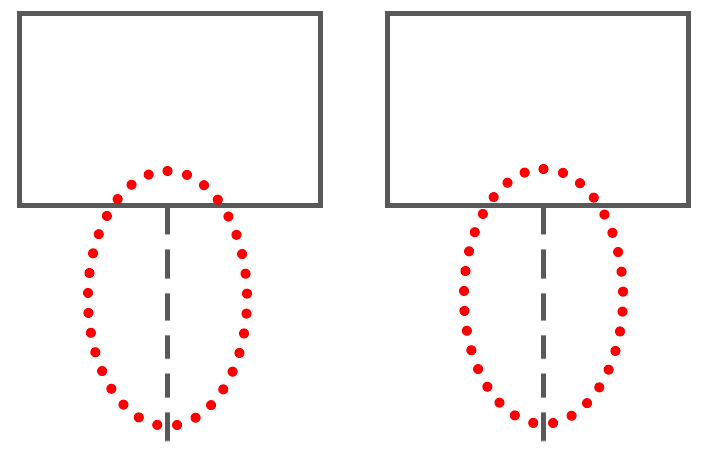
\includegraphics[width=2.3in]{uml-lifeline}} & lifeline &  Vertical dashed line representing the lifespan of the participant. Top is beginning of life, bottom is end. Life ends when the participant is deleted.\\
\raisebox{-\totalheight}{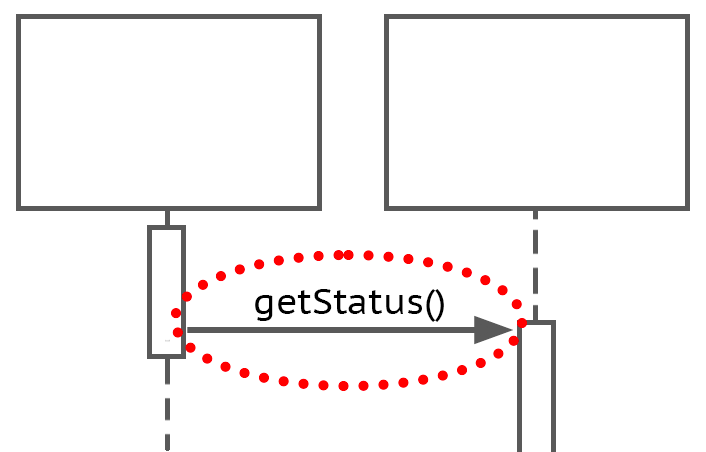
\includegraphics[width=2.3in]{uml-message}} & message & Interaction from one participant to another. Solid line with arrow. Often a method call.\\
\raisebox{-\totalheight}{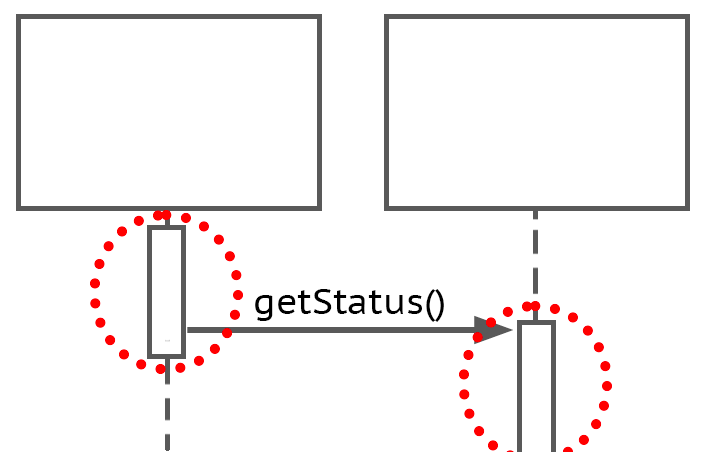
\includegraphics[width=2.3in]{uml-activation}} & activation & Box on lifeline indicating when the participant is active. Indicates method is on call stack.\\
\raisebox{-\totalheight}{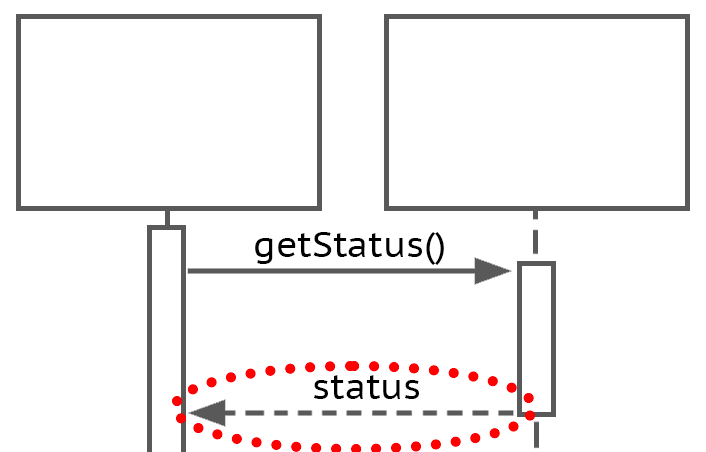
\includegraphics[width=2.3in]{uml-return}} & return & Dashed line with arrow indicating method return. Use only when it helps communicate something important about the interaction.\\
\end{tabular}

\rowcolors{2}{gray!25}{white}
\noindent\begin{tabular}{p{2.5in} p{1in} p{2.5in}}
\rowcolor{gray!25}
\raisebox{-\totalheight}{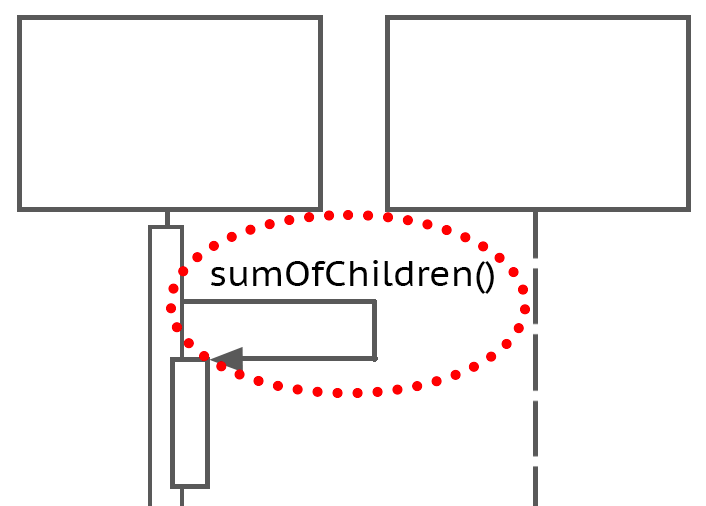
\includegraphics[width=2.3in]{uml-selfcall}} & self-call & Method calling self. Solid line with arrow pointing back to participant's own lifeline.\\
\raisebox{-\totalheight}{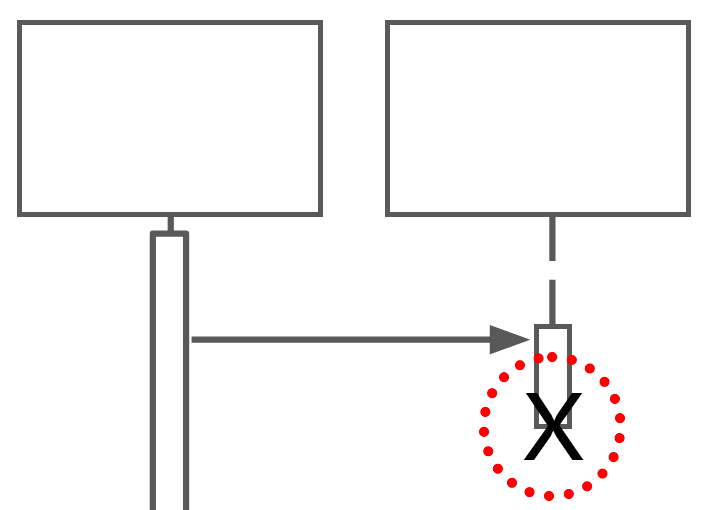
\includegraphics[width=2.3in]{uml-deletion}} & deletion & End of participant's life. Indicated by ``X'' on lifeline. \\
\end{tabular}

\section{Conclusion}
UML diagrams can be helpful for communicating how your code works. Class diagrams and sequence diagrams are two common-used types of UML diagrams. Each type of diagram emphasizes some part of the code design while leaving out other parts. This is because UML diagrams are for communicating with humans---not computers.

\section{Additional Resources}

\begin{description}
\item \fullcite{miles2006learning}
\item \fullcite{fowler2003uml}
\end{description}
\yesmargins

\chapter{Monolith vs. Microservices Architectures}
\chaptermark{Monolith vs. Microservices}

\begin{tikzpicture}[overlay,remember picture] 
\node[anchor=south] at ([yshift=5in,xshift=0.85in]current page text area.south){\includegraphics[width=9.5in]{msa05}}; 
\end{tikzpicture}

\marginpar{\softwareArchitectureDef\margindivider}

\marginpar{\highLevelArchitectureDef}

\textbf{High-level architecture} is the software's all-encompassing code design. When described with the diagram, a high-level architecture usually looks like a few to dozens of interconnected shapes with short labels, an abstraction that usually represents the entire codebase. In this chapter, we'll use ``\textbf{architecture}'' interchangeably with ``high-level architecture'' (in other contexts, architecture can refer to code design at lower levels).

If you're developing new software, you might get to choose the high-level architecture, or it may already be baked into a framework you've chosen. For example, many web application frameworks use the Model-View-Controller (MVC) architecture or variants. In the latter case, you have to learn MVC and how to work within it; The design decision is made for you.

\marginpar{\monolithArchitectureDef\margindivider}\marginpar{\microservicesArchitectureDef\margindivider}\marginpar{\abstractionDef}Since my aim is to help you make choices about software, I \textbf{won't be covering every high-level architecture}. Instead, I'll concentrate on two distinct high-level architectures: \textbf{monolith} and \textbf{microservices}. Talking about the ways they're different will lead us through concepts applicable to architectures in general.

\section{Monolith Architecture}

\textbf{Monolith} software is one or few pieces and \textbf{cannot easily be divided} into multiple independent components that run separately and are individually useful. What about when the client side, the server side, and the database are all separate, can that be a monolith? Yes. If the client-side part of the software will not start or is not useful without the database or server-side part of the software, that's a monolith.

If you're trying to think of an example of a monolith and nothing is coming to mind, that's probably because this architecture is so common; it can arise without having to plan. Your first computer program was probably a small monolith. If you keep adding more code / files / classes / components, the software becomes a bigger monolith---unless you make a different design decision.

\section{Microservice Architecture}

\textbf{Microservices} are \textbf{multiple pieces} of software, each of which runs in a \textbf{separate process} and can be \textbf{individually useful}. This section describes core characteristics of software that uses the microservice architecture. Additional commentary from Lewis and Fowler at \parencite{fowler2019microservices}. 

\subsection{``Smart endpoints and dumb pipes''}
\marginpar{``Dumb pipes'' does not imply simple message contents.}
The \textbf{communication pipe} within microservice architectures is \textbf{simple} and the services themselves take care of translating and otherwise processing messages. For example, microservices commonly communicate through a REST API, which allow these kinds of messages: GET, POST (create), PUT (update), or DELETE. The contents of the messages can be complex but it's the job of the services to deal with that.

\subsection{``Componentization via services''}\marginpar{\componentDef\margindivider}\marginpar{\serviceDef\margindivider}\marginpar{Even though it provides a service, a library is not a service if you're including its code in your code.\margindivider}\marginpar{\couplingDef\margindivider}\marginpar{\encapsulationDef}

In a microservice architecture, \textbf{components are services}. The Lewis and Fowler definition of a \textbf{component} is, ``a unit of software that is independently replaceable and upgradeable''. A \textbf{service} provides functionality while running in its own process. In a monolith, it's more common to have more \textbf{tightly coupled} code and components that run in the same process.

\spacer
\noindent\textbf{Advantages of splitting components into services:}\\

\begin{itemize}
    \item \textbf{Independence}: Each individual service can be updated, tested, launched, and stopped without requiring the same from other parts of the software. In contrast, with some monolithic software, for example, all tests must be run each time a developer commits to a change, which can make for a long wait. If a service fails, any software depending on it will be without that service but the rest of the software needn't be affected.\\
    \item \textbf{Standardized component communication}: Service communication pipes can be simple and the same each time. This can make for less thinking, fewer mistakes, and less violation of \textbf{encapsulation} when connecting two components---just use the pipe.
\end{itemize}

\spacer
\noindent\textbf{Disadvantages of splitting components into services:}\\

\begin{itemize}
    \item \textbf{More expensive communication}: Whereas in a monolith communication between components can be direct calls (fast, light-weight), with microservices \textbf{requests} often happen \textbf{over a network}, need to include metadata to explain the request, and, because the pipes are ``dumb'', responses can contain extra data the requester didn't ask for (slower, heavier).\\
    \item \textbf{Potentially less secure communication}: Communication over a network can be more prone to interception and alteration.
\end{itemize}

\subsection{``Organized around business capabilities''}\marginpar{\clientServerArchitectureDef\margindivider}\marginpar{\businessCapabilityDef\margindivider}\marginpar{In each of these examples, what are the business resources producing customer value? What is the value to the customer? How are the business resources acting on their environment? What other resources are the business resources using?\margindivider}\marginpar{\eventualConsistencyDef\margindivider}\marginpar{\techStackDef}

You may have heard of the \textbf{client-server high-level architecture}, which usually consists of multiple instances of client-side software that communicate with server-side software, which communicates with a database. That architecture is organized around technology. Another way to put that: Someone unfamiliar with the differences between client-side software, server-side software, and a database would not get much out of seeing a diagram of this architecture. 

In contrast, microservices are organized around \textbf{business capabilities}. This term has multiple definitions. Michell's integrated definition fits what we're talking about: ``the potential of a business resource (or groups of resources) to produce customer value by acting on their environment via a process using other tangible and intangible resources'' \parencite{Michell2011AFA}. 

\spacer
\noindent\textbf{Examples of business capabilities:}\\

\begin{itemize}

\item The manufacturer can slice a 20ft by 40ft rectangle of wheat dough into 0.5cm strips in 1.2 seconds, which will later become packaged noodles someone can buy for lunch in a grocery store.

\item A loan officer can lead a customer through the process of securing a loan, enabling the customer to start a small business.

\item A pet food distributor can regularly ship nutritionally-balanced cat food to stores around the country.

\item The software can convert a video so it works better on mobile devices.

\end{itemize}

\spacer
One implication of being focused on business capabilties is that each microservice has its own \textbf{tech stack} (including its own database).

\nomargins
\subsection{``Decentralized data management''}

In a \textbf{microservice} architecture, each service \textbf{typically has its own database} instead of sharing a centralized database. This helps keep the microservices independent, which has many benefits including \textbf{failure containment}. A disadvantage is that interoperating microservices can end up with copies of the same data that are inconsisent (e.g., because one database has not yet received the update). The term for this is \textbf{eventual consistency}, which means that, with time, each microservice will have the most up-to-date information but meanwhile there could be a mismatch (perhaps one that will annoy or mislead human users).

\subsection{``Decentralized governance''}

Microservices need only be compatible at their interfaces (communication pipe), leaving \textbf{flexibility in how each is implemented}. For example, each service can be written in a different language, reducing the weight of \textbf{tech stack} decisions and decreasing the need to compromise on those decisions: For each service, teams can choose the optimal programming language, framework, architecture, etc. If, later, the team needs to change to different technologies, only the one service is affected. On the other hand, in a monolith, teams might only need to maintain a small set of technologies (e.g., if there's only one framework, only one framework will need updates installed) and might not need as broad of expertise (e.g., having working knowledge of five programming languages). Also, when code is more-or-less part of the same codebase, it might be easier to maintain the same standards across the code.

\subsection{``Design for failure''}

When services running in different processes on different machines and potentially being written with different technologies by different teams with different standards, that \textbf{can change how developers think}. Instead of keeping the whole ship afloat, thinking can shift toward what to do if a service fails. With that comes \textbf{monitoring}, \textbf{logging}, and design decisions about \textbf{what to do when a service fails}---including what to tell the user. In contrast, with a monolith, more thought might be put into how to revert quickly if a deployment fails (because failure might mean no part of the monolith works). Monoliths can also be designed for failure but that's not as natural a tendency as with microservices.

\section{Comparison Between Monolith and Microservices}

This section recaps and expands upon differences between monolith and microservice architectures.

\subsection{How does communication happen within a monolith versus between microservices?}
In a \textbf{monolith}, \textbf{communication} (e.g., between classes and components) can happen in many ways, including through \textbf{direct calls} and over a network. With \textbf{microservices}, communication typically happens \textbf{over a network} such as through HTTP requests/responses, through ``dumb'', standardized communication pipes. While microservices communication \textbf{pipes are less complex}, that means the endpoints need to be smarter. Also, \textbf{communication over a network can be less reliable}.

\subsection{How is a monolith deployed vs. microservices?}

\textbf{Monolithic} software \textbf{often needs to be deployed all at once}. \textbf{Microservices} can be \textbf{independently deployed}, and can potentially be stopped without stopping connected services.

\subsection{How is a monolith scaled vs. microservices?}

If your \textbf{monolithic} software needs more resources to be able to support how much it's being used, it can be \textbf{copied onto multiple machines}. Each machine must have enough s\textbf{pace, memory, processing} speed, etc. to support the entire monolith.

If your \textbf{microservices} software needs more resources, you have more options. For example, the \textbf{services that are used more can be replicated more} times.

\subsection{How is a monolith tested vs. microservices?}

In \textbf{microservice} software, each service can be \textbf{independently tested}. In a \textbf{monolith}, the way you test is \textbf{influenced by dependencies} within the code, which could reach broadly across the software (and make for \textbf{slow tests}).

\subsection{How is a monolith upgraded vs. microservices?}

Each \textbf{microservice} can be written in a \textbf{different language} (e.g., one in Python, another in Java, another in C++, etc.), and can run in different contexts (e.g., machines with different operating systems, libraries, versions of libraries, etc.). \textbf{In theory}, this means they can be \textbf{independently upgraded}.

With a \textbf{monolith}, upgrading \textbf{may require more care}; each component must be compatible with the new context (but this is also sometimes true with microservices).

\subsection{How is the database used in a monolith vs. microservices?}

\textbf{Monolithic} software \textbf{might have just one database}, potentially a very large one. This can create a \textbf{bottleneck} if multiple parts of the software need to access the database in parallel and can make for slow database backing up and restoring, among other drawbacks. However, if you only have one database, that's \textbf{just one place for managing} database access accounts and one database to maintain / back up / restore / etc. In contrast, \textbf{each microservice} typically has its \textbf{own data storage}.

\section{Conclusion}
The \textbf{microservices} architecture has advantage of being \textbf{modular}, where each service can be independently-managed. Communication mechanisms between modules can be \textbf{standardized}. However, creating a \textbf{monolith} can require \textbf{less planning} ahead of time and modules within a monolith can \textbf{communicate directly}, which can be \textbf{more reliable, less expensive, and provide better consistency} than communicating to many pieces of software through a network.

\section{Additional Resources}

\begin{description}
    \item \fullcite{fowler2011tolerant}
    \item \fullcite{fowler2015microservices}
    \item \fullcite{fowler2019microservices}
    \item \fullcite{ibm2021http}
    \item \fullcite{ibm2021esb}
    \item \fullcite{ibm2021rest}
    \item \fullcite{Michell2011AFA}
    \item \fullcite{mozilla2021http}
    \item \fullcite{newman2015building}
\end{description}

\yesmargins
\input{uip}
\yesmargins
\chapter{Cognitive Style Heuristics}
\begin{tikzpicture}[overlay,remember picture] 
\node[anchor=south] at ([yshift=5in,xshift=2.1in]current page text area.south){\includegraphics[width=11.5in]{csh02-sm}}; 
\end{tikzpicture}\marginpar{\cognitiveStyleHeuristicsDef\margindivider}\marginpar{\interactionDesignDef}The \textbf{Cognitive Style Heuristics (CSH)}\index{cognitive style heuristics} are eight principles of \textbf{interaction design}\index{interaction design} used to improve software usability\index{usability}. They are framed around how different people use software in different ways. The CSH\index{cognitive style heuristics} were created by a research team headed by Margaret Burnett, one of the world's leading experts in usability research and \textbf{inclusive software design}.

The CSH\index{cognitive style heuristics} were created with new users in mind: People who have never seen, interacted with, or received previous direction on the software. They can also improve usability for more seasoned users who have figured out how to use the software to complete their tasks but may still be unhappy with the software.

\section{Cognitive Style Facets}\marginpar{\inclusiveSoftwareDesignDef\margindivider}\marginpar{\cognitiveStyleFacetsDef\margindivider}\marginpar{\motivationCsfDef\margindivider}\marginpar{\informationProcessingStyleCsfDef\margindivider}\marginpar{\computerSelfEfficacyCsfDef}

At the core of the Cognitive Style Heuristics\index{cognitive style heuristics} are the \textbf{cognitive style facets}\index{cognitive style facets}, five aspects of human cognition that affect how users problem-solve in software:

\begin{enumerate}
\item{\textbf{Motivations} for using software (task completion vs. tech interest). A person who is feeling task-motivated might choose to use software because they have something specific they need to accomplish, and might focus on that task immediately when they open the software and the whole time they're using it. A person who is feeling interested in the software itself might seek out the new and exciting features and spend a lot of time exploring them.}

\item{\textbf{Information processing style} (comprehensive vs. selective). A person processing comprehensively might want to understand details, implications, or to get a sense of overall structure before taking action in software. A person processing selectively might take action as soon as they detect what seems like the beginning of a promising path.}
\item{\textbf{Computer self-efficacy} (low vs. high). A person who is feeling low computer self-efficacy might think it's their fault when they make a mistake or encounter a problem in the software. A person feeling high computer self-efficacy might feel the software is poorly made if they make a mistake or encounter a problem in the software.}
\item{\textbf{Attitude toward risk} (risk-tolerant vs. risk-averse). A person who is feeling risk-averse might avoid taking actions that have unknown consequences or seem dangerous or irreversible. A person who is feeling risk-tolerant might take actions even if they know those actions could lead to bad consequences.}
\item{\textbf{Learning style} (tinkering vs. by process). When someone is tinkering, they might click a button just because it's clickable then learn from what happens. When someone is learning by process, they might seek a logical first step, and want to proceed smoothly from start to finish.}
\end{enumerate}

As you probably noticed, each of the cognitive style facets has two polar \textbf{cognitive style facet values} (or \textbf{cognitive styles}\index{cognitive styles}). Each pair of facet values creates a spectrum. When each of us uses software, the way we feel and behave corresponds to somewhere on each of those spectra. Our individual facet values may be similar each time we use software, but they can also vary by context and change over time. For example, many people feel cognitively impatient when reading paragraphs of text (``text walls'') on websites and might process them more selectively, whereas they might want to catch every word of a new novel by their favorite author (comprehensive processing). \marginpar{\attitudeTowardRiskCsfDef\margindivider}\marginpar{\learningStyleCsfDef\margindivider}\marginpar{\cognitiveStyleFacetValueDef\margindivider}\marginpar{\personaDef\margindivider}\marginpar{\cognitiveStylePersonasDef}

\section{Cognitive Style Personas}

The CSH are stated from the perspective of improving usability for the three \textbf{cognitive style personas}: Abi, Pat, and Tim. A \textbf{persona}\index{persona} is fictional person that is created to represent a group of users within a target audience. Personas are used to help marketing teams keep important subsets of their target audience in mind, and in software UI design for the same reason. Personas are typically documents that include a photo, name, age, gender, other background information, and information about how the made-up person interacts with product or software.

The cognitive style personas have a similar purpose but are distinct from traditional personas in multiple ways:
\begin{itemize}
\item{There are three and only three (Abi, Pat, and Tim).}
\item{Abi, Pat, and Tim each have a different set of cognitive styles. The cognitive styles are fixed.}
\item{Abi, Pat, and Tim are each multi-personas: They each have multiple photos of different people who appear to be of different ages, races, genders, etc.}
\item{Abi, Pat, and Tim were specifically created for evaluating \textit{software} (not marketing).}
\item{Abi, Pat, and Tim represent different positions on the cognitive style facet spectrum: Abi and Tim are on the ends and Pat is in the middle.}
\end{itemize}

The idea of the cognitive style personas is that creating software that works well for Abi and Tim (the two ends of the cognitive style facet value spectrum) will result in software that's better for them and everyone in between.

\nomargins
\subsection{Abi, Pat, and Tim}

\begin{tcolorbox}[colback=abicolor!100!white,colframe=abicolor2!100!black]
{\Large \textbf{Abi (Abigail/Abishek)}}\\
\includegraphics[scale=0.5]{abi1}
\includegraphics[scale=0.5]{abi3}
\includegraphics[scale=0.5]{abi2}\\
\textbf{Motivation}: Uses technology to accomplish their tasks.\\
\textbf{Computer self-efficacy}: Lower self-confidence than their peers about doing unfamiliar computing tasks. Blames themselves for problems.\\
\textbf{Attitude toward risk}: Risk-averse about using unfamiliar technologies that might require a lot of time\\
\textbf{Information processing style}: Comprehensive\\
\textbf{Learning style}: Process-orientated learning
\end{tcolorbox}

\begin{tcolorbox}[colback=patcolor!100!white,colframe=patcolor2!100!black]
{\Large \textbf{Pat (Patricia/Patrick)}}\\
\includegraphics[scale=0.5]{pat2}
\includegraphics[scale=0.5]{pat1}
\includegraphics[scale=0.5]{pat3}\\
\textbf{Motivation}: Learns new technologies when they need to\\
\textbf{Computer self-efficacy}: Medium confidence doing unfamiliar computing tasks. If a problem can't be fixed, they will keep trying\\
\textbf{Attitude toward risk}: Risk-averse and doesn't want to expend time when they might not receive benefits\\
\textbf{Information processing style}: Comprehensive\\
\textbf{Learning style}: Likes to explore and purposefully tinker
\end{tcolorbox}

\begin{tcolorbox}[colback=timcolor!100!white,colframe=timcolor2!100!black]
{\Large \textbf{Tim (Timara/Timothy)}}\\
\includegraphics[scale=0.5]{tim1}
\includegraphics[scale=0.5]{tim3}
\includegraphics[scale=0.5]{tim2}\\
\textbf{Motivation}: Likes learning all the available functionality on all their devices\\
\textbf{Computer self-efficacy}: High confidence in technical abilities. If a problem can't be fixed, blame goes to software vendor.\\
\textbf{Attitude toward risk}: Doesn't mind taking risk using features of technology\\
\textbf{Information processing style}: Selective\\
\textbf{Learning style}: Likes tinkering and exploring
\end{tcolorbox}

\section{The Heuristics}

Adapted from \parencite{burnett2021heuristics}.\\

\noindent\textbf{Note}: The designs shown below were modelled after examples found in published software.

\subsection{Heuristic \#1 (of 8): Explain the \textit{benefits} of using new and existing features}

\begin{itemize}
\item \textbf{Abi and Pat are task-motivated} so might lose interest if they don't see how a feature relates to their task.
\item \textbf{Abi is risk-averse} so might avoid features with too many unknowns.
\item \textbf{Tim is risk-tolerant} and \textbf{motivated by tech interest} so might take a chance on features then be disappointed at how mundane they are.
\end{itemize}

\noindent To support users' motivations and attitudes toward risk, \textbf{provide Abi and Pat ways to decide whether a feature relates to their task and provide Tim ways to decide whether a feature is new and unique}.

\spacer
\noindent\textbf{Example 1: Each featured extension has a brief description that says what the extension does and why somebody would use it.}
\begin{center}
\noindent\includegraphics[width=0.95\textwidth]{h1-03}
\end{center}

\noindent\textbf{Example 2: Announcement briefly describes a new feature and how to use it.}
\begin{center}
\noindent\includegraphics[width=0.95\textwidth]{h1-04}
\end{center}

\noindent\textbf{Example 3: Tooltip says why someone might use the search.}
\begin{center}
\noindent\includegraphics[width=0.7\textwidth]{h2-03}
\end{center}

\noindent\textbf{Example 4: Each tile explains a feature and the benefit of using the feature.}
\begin{center}
\noindent\includegraphics[width=0.95\textwidth]{h2-04}
\end{center}

\subsection{Heuristic \#2 (of 8): Explain the \textit{costs} of using new and existing features}

\begin{itemize}
    \item Abi and Pat are risk-averse, so they may want to avoid features with high effort costs if the benefits of using these features are unclear.
    \item Tim is risk-tolerant, so may begin using features that require extra effort and time, and that are unrelated to the task at hand.
\end{itemize}

\noindent To support their \textbf{attitudes toward risk}, allow Abi and Pat to decide whether or not a feature will require too much effort to use. To help Tim stay on track with their task, allow them to understand that a feature may take extra effort, and thus more time.

\spacer
\noindent\textbf{Example 1: Placing ``Advanced Options'' at the bottom of the menu indicates to the user that ``advanced'' features may take more effort.}\\
\begin{center}
\noindent\includegraphics{h7-03}
\end{center}

\noindent\textbf{Example 2: The dialog indicates that ``cor launcher'' will be needed to ``associate files with Coral'' and that the user will need write permissions for the installation folder.}\\
\begin{center}
\noindent\includegraphics{h7-04}
\end{center}

\subsection{Heuristic \#3 (of 8): Let people gather as much information as they want, and no more than they want}

\begin{itemize}
\item Abi and Pat gather and read relevant information comprehensively before acting.
\item Tim likes to delve into the first option and pursue it, backtracking if need be.
\end{itemize}

\noindent To support their \textbf{information processing styles}, allow Abi and Pat to easily obtain as much information they want, but don't require them to spend excessive time or effort gathering that information. Allow Tim to get to directly useful information immediately so that they can act upon it without wading through a lot of information they don’t want.

\spacer
\noindent\textbf{Example 1: Users can choose to view code documentation while still viewing their code.}
\begin{center}
\noindent\includegraphics{h3-03}
\end{center}

\noindent\textbf{Example 2: Users can quickly see the contents of the webpage and jump to the section they're interested in.}
\begin{center}
\noindent\includegraphics{h3-04}
\end{center}

\subsection{Heuristic \#4 (of 8): Keep familiar features available}

\begin{itemize}
\item Abi has lower computer self-efficacy and is more risk-averse than Tim, so if a problem arises when they are trying to use an unfamiliar feature, Abi blames themself and stops using the tech rather than potentially wasting their time trying to get the unfamiliar feature working.
\item Pat has medium self-efficacy with technology, so if a problem arises when they are trying to use an unfamiliar feature, Pat will try alternative ways of succeeding for a while. However, Pat is also risk-averse so prefers to perform tasks using familiar features, because they're more predictable about what Pat will get from them and how much time they'll take.
\item Tim has higher computer self-efficacy and is more risk-tolerant than Abi, so if a problem arises when they are trying to use an unfamiliar feature, they’ll blame the tech, and may spend a lot of extra time trying to work around a problem in numerous ways.
\end{itemize}

\noindent To support their \textbf{computer self-efficacies} and \textbf{attitudes toward risk}, and to encourage Abi, Pat, and Tim to keep using the tech without wasting their time, enable them to interact with it using the same features they’ve used in the past.

\spacer
\noindent\textbf{Example 1: Although the ``following'' page is gone, the new update looks similar to the previous version so that users are still familiar with the app.}
\begin{center}
\noindent\includegraphics[width=0.7\textwidth]{h4-03}
\end{center}

\noindent\textbf{Example 2: The smartphone and tablet versions of this app offer the same features which makes switching between the two easy.}
\begin{center}
\noindent\includegraphics[width=0.7\textwidth]{h4-04}
\end{center}

\subsection{Heuristic \#5 (of 8): Make undo/redo and backtracking available}

\begin{itemize}
\item Abi and Pat are risk-averse, so they prefer not to take actions in technology that might not be easy to reverse.
\item Tim is risk-tolerant, so is willing to take actions in technology that might be incorrect and need to be reversed.
\end{itemize}

To support their \textbf{attitudes toward risk}, provide undo/redo and backtracking to allow Abi and Pat to feel comfortable proceeding with actions whose consequences may not be clear, so that that they know they can easily reverse these actions, and so that Tim can recover from mistakes.

\spacer
\noindent\textbf{Example 1: Browser back/forward buttons allow users to backtrack through their browsing history.}\\
\begin{center}
\noindent\includegraphics{h5-03}
\end{center}

\noindent\textbf{Example 2: An undo button allow users to make and recover from mistakes. Also, version control systems allow users to revert to any previously-committed code state.}\\
\begin{center}
\noindent\includegraphics{h5-04}
\end{center}

\subsection{Heuristic \#6 (of 8): Provide an explicit path through the task}

\begin{itemize}
\item Abi is a process-oriented learner, so prefers to proceed through tasks step-by-step.
\item Tim and Pat learn by tinkering, and therefore prefer not to be constrained by rigid, pre-determined processes.
\end{itemize}

\noindent To support their \textbf{learning styles}, explicitly provide Abi a clear process to go through the task, and provide Tim and Pat a way to bypass step-by-step processes and tutorials if those are not required for learning the technology.

\spacer
\noindent\textbf{Example 1: Users can choose their entry point, and each path is explained.}\\
\begin{center}
\noindent\includegraphics{h8-03}
\end{center}

\noindent\textbf{Example 2: Users get to choose either the path of learning more about the new feature or going back to what they were doing.}\\
\begin{center}
\noindent\includegraphics{h8-04}
\end{center}

\subsection{Heuristic \#7 (of 8): Provide ways to try out different approaches}

\begin{itemize}
\item Abi has lower computer self-efficacy than Tim, so if a problem arises when they are trying to use technology, Abi blames themself and stops using the tech.
\item Pat has medium self-efficacy with technology, so if a problem arises when they are trying to use technology,  Pat will try alternative ways of succeeding for a while.
\item Tim has higher computer self-efficacy than Abi, so if a problem arises when they are trying to use technology, they’ll blame the tech, and then will try numerous workarounds to get around the problem.
\end{itemize}

\noindent To support their \textbf{computer self-efficacies}, point Abi toward a different approach when they feel unable to proceed with the current one. This will also point Tim and Pat to multiple ways they can try to solve the problem.

\spacer
\noindent\textbf{Example 1: If users don't find what they need on the ``Choose a Question'' drop-down menu, they can try the chat.}\\
\begin{center}
\noindent\includegraphics{h6-03}
\end{center}

\noindent\textbf{Example 2: If users encounter a problem using the SecureChat UI, they can attempt the same operations using the command line interface.}\\
\begin{center}
\noindent\includegraphics{h6-04}
\end{center}

\subsection{Heuristic \#8 (of 8): Encourage tinkerers to tinker mindfully}

\begin{itemize}
\item Tim learns by tinkering, but sometimes tinkers addictively and gets distracted from their task.
\item Pat learns by trying out new features but does so mindfully, reflecting on each step.
\end{itemize}

\noindent To support their \textbf{learning styles}, encourage Tim not to over-tinker (e.g., by adding an extra click), so that they make fewer mistakes, have time to absorb important information, and stay on-task.

\spacer
\noindent\textbf{Example 1: This design encourages users to tinker mindfully by showing they will notify them before impactful actions are executed, like emailing 237 people.}\\
\begin{center}
\noindent\includegraphics{h9-03}
\end{center}

\noindent\textbf{Example 2: This design encourages users to try out new ``slash'' commands by showing all the commands when a user types ``/'', and explaining what each does and how to use it.}\\
\begin{center}
\noindent\includegraphics{h9-04}
\end{center}

\yesmargins
\section{Background}

\marginpar{\heuristicEvaluationDef\margindivider}

\marginpar{The cognitive style personas are simplified versions of the GenderMag personas. You can find the the GenderMag personas, and a full description of their research origins, at \href{http://gendermag.org/}{GenderMag.org}\margindivider}

\marginpar{\genderMagMethodDef\margindivider}

\marginpar{\cognitiveWalkthroughDef}

The Cognitive Style Heuristics are meant to be used in a \textbf{heuristic evaluation}\index{heuristic evaluation}, a process where software designers or evaluators go through heuristics one-by-one like a checklist, deciding whether the design does or does not reflect the heuristic. The evaluation is done independently by two or more people, who then compare findings.

The Cognitive Style Heuristics are derived from the GenderMag Heuristics \parencite{gendermagheuristics} and the \textbf{GenderMag Method} \parencite{burnett16}. The GenderMag Method is a process for finding and fixing gender-inclusivity bugs in software. Instead of heuristic evaluation, it uses a \textbf{cognitive walkthrough}. It uses the same personas: Abi, Pat, and Tim. However, in addition to their cognitive styles, each GenderMag persona has additional sections, such as one with customizable background information.

What do cognitive styles have to do with gender? Software tends to be biased against the cognitive styles often favored by women. Designing with cognitive styles in mind can make software less gender-biased \parencite{vorvoreanu19}.

In addition, ``designing software so that it works for diverse populations matters to software companies’ profitability, to equity in the workplace and at home, and to anyone in a situation that changes the way they think, such as when under deadline pressure.''\parencite{mendez19}

\section{Conclusion}

The Cognitive Style Heuristics are a set a eight software usability heuristics for evaluating and improving the usability of UIs across users with different cognitive styles.

\nomargins
\section{Additional Resources}

\begin{description}
\item \fullcite{burnett16}
\item \fullcite{hill2017gender}
\item \fullcite{gendermag}
\item \fullcite{gendermagheuristics}
\item \fullcite{martin12}
\item \fullcite{mendez19}
\item \fullcite{nielsen90}
\item \fullcite{nielsen94}
\item \fullcite{norman13}
\item \fullcite{pruitt10}
\item \fullcite{vorvoreanu19}
\end{description}
\yesmargins

\chapter{Code Smells and Refactoring}

\begin{tikzpicture}[overlay,remember picture] 
\node[anchor=south] at ([yshift=5in,xshift=0.85in]current page text area.south){\includegraphics[width=9in]{smells01}}; 
\end{tikzpicture} 

\textbf{Code smells}\index{code smells} are aspects of code that indicate the code needs to be reorganized---signs your software is \textbf{decaying}\marginpar{\codeSmellDef\margindivider}\marginpar{\codeDecayDef}. Your code might need attention if you're having thoughts like these:

\begin{itemize}
\item ``I would \textbf{never show this code} during an interview.''
\item ``I'm going to \textbf{start over} and re-write this code from scratch.''
\item ``Every time I look at this code, I have to \textbf{re-figure-out} what it does.''
\item ``I \textbf{don't} think these code comments \textbf{match} what the code is doing...''
\item ``Why is this code \textbf{repeated} in three different places?''
\item ``I want to switch out this component, but \textbf{that'll break} X, Y, and Z in this other place and I don't want to deal with that.''
\end{itemize}

Types of codes smells we'll cover (including how to fix them):\\

\begin{itemize}
\item Code smells about \textbf{comments}
\item Code smells about \textbf{functions}
\item \textbf{General code} smells (e.g., about the code within functions)\\
\end{itemize}

\marginpar{If you want to learn more about any of the code smells and refactorings\index{refactoring} described in this chapter, or want to know MORE ways your code can smell, \parencite{martin13} and \parencite{shvets21} are two good resources.}

\section{Why care about code smells?}\index{code smells}

\textbf{Reasons} to pay attention to and fix code smells:\\

\begin{itemize}
\item Smelly code can be \textbf{harder for you and others to maintain} because the code is unclear. When code is hard to maintain, developers tend to work around it or re-create the same functionality elsewhere.\\
\item Smelly code \textbf{leads to smellier code}. When you let your code become disorganized, you are giving yourself and others the message that smelly code is acceptable. Disorganized code also tends to give us an excuse to be lazy coders. A web development example: If you've used CSS, you may have encountered frustrating situations where the style you're trying to apply is not working---somewhere in the code (e.g., other CSS, HTML, or JS), your style is being overridden. Instead of tracking down the competing code or markup, you use the ``!important'' property which forces the style to be applied. The codebase is a mess anyway, so who cares? Your future self.\marginpar{If you think it's more fun to write code than organize code, you may need to be strict with yourself about using good programming practices.}\\
\item Smelly code builds up \textbf{technical debt}\index{technical debt}. If the code is working, there's never a reason to change it, right? Wrong. Each time you write sloppy code, you are contributing to your project's technical debt. Maybe it works now but, as sloppy software grows, it will get more difficult to deal with. That can mean your company needing to hire more developers to keep productivity up. Instead, productivity can go down because now the old developers are struggling to teach the new developers and everyone is continuing to write sloppy code. Ultimately, the software may have to be redeveloped entirely (which doesn't always solve the problem). Or, the project could fail.
\end{itemize}

\section{Your code stinks, now what?}

If you're in a position to (e.g., your manager allows it), strongly consider \textbf{refactoring}. Refactoring\index{refactoring} is when you improve your code without changing what the code does. Refactoring is how you fight against technical debt\index{technical debt}.\marginpar{\refactoringDef\margindivider}\marginpar{\technicalDebtDef}

The remainder of this chapter is about code smells and how to clean them up. This is not an exhaustive list. You can find a lot more by looking through the resources listed at the end of this chapter.

\section{Comments}

When we first learned to code, many of us didn't write comments: solving problems is fun and coding can be addictive, no time for boring comments! Then, we got more experience, started coding with others, were formally trained on coding, or attempted to pick up an old project, and we saw why comments are useful---and then some of us jumped to the other extreme: too many comments. We explained functions with paragraphs of prose, or even commented each line. It's tedious, but it's the right thing to do, right? Unfortunately (and fortunately), \textbf{too many comments can be as bad as none}.

\subsection{Drawbacks of Having Many Comments}\marginpar{Don't fall into the trap of adding excessive comments to your code before an interview! Some prospective employers specifically look for over-commented code (or can't help but see it) as a indicator of poor programming habits.}

\begin{itemize}
\item {Comments \textbf{get out of date quickly}. If we update the code, then procrastinate on the comments, what we leave can be misleading (to others and our future selves). Also, more comments means greater likelihood some will be neglected, giving us the smelly situation of some accurate and some inaccurate comments. In that case, why would we trust \textit{any} of the comments?\\}
\item{Writing comments for straightforward code \textbf{can distract from the important comments}. If the code was difficult to write, is long, is unique, is complex, or has a ``gotcha'', that code is more important to call attention to with comments.\\}
\item{Writing lots of comments could \textbf{indicate the code needs to be simplified}. Ideally, most of the the code you write will be self-explanatory so that comments are infrequently needed.}
\end{itemize}

\subsection{Code Smells about Comments}

Below is a concise \textbf{list of common code smells}\index{code smells} about comments and what to do about them (how to refactor).\\

\begin{itemize}
\item {
\textbf{Obsolete Comment} (no longer describes the code).\\
Remove or update.
\lstinputlisting[language=Python]{code/csr-comments-obsolete.py}\spacer
}
\item {
\textbf{Commented-Out Code} (somebody thought they'd need that code later, but the commented out block is now getting out of date and in the way).\\
Remove. If you're feeling risk-averse, save a backup or use a version-control system.\marginpar{As a challenge to myself, I kept the code example boxes narrow and tried to make the ``good'' code fit.\margindivider}\marginpar{Commenting out code often comes with poor assumptions (e.g., you'll need the code later, others will understand why you commented it out, the surrounding code will continue having the same purpose, etc.)}
\lstinputlisting[language=Python]{code/csr-comments-deadcode.py}\spacer
}
\item {
\textbf{Redundant Comment} (states what would already be immediately apparent to a programmer of any level).\\
Remove. Less is more.
\lstinputlisting[language=Python]{code/csr-comments-redundant.py}\spacer
}
\item {
\textbf{Long Comment} (multiple sentences, complicated, goes into a lot of detail)\\
Simplify the code to make it more self-explanatory, shorten or remove comment.
\lstinputlisting[language=Python]{code/csr-comments-long.py}\spacer
}
\end{itemize}

\section{Functions}

\marginpar{If you're only writing a short program, does coding style matter? Treating code as disposable is a self-fulfilling prophecy.}A natural way to code is to start writing a function and then, as the program gets more complicated, keep adding to it. For example, if your program's GUI only has a start and a stop button, the function for populating the screen with UI elements need only draw those two buttons. Then, when you add a menu and a settings button, you could update the function to draw those elements, too. Then you add user accounts and decide that function is a fine place to check if the user is logged in, their level of inactivity, show a pop-up about cool new features... and your function balloons. Understanding the small details of how the function works can even make one feel proud---until the \textbf{code becomes unmaintainable and bug-ridden}.  

\subsection{Code Smells about Functions}

\marginpar{Software made of 3 to 4-line functions is amazing to behold!}Follow these \textbf{refactoring suggestions} to increase code readability, maintainability, and modularity.\\

\begin{itemize}

\item{\textbf{Long Function} (more than 10 lines or so)\\Break into multiple functions. Aim for five lines or fewer.\\}

\item{\textbf{Function with Many Jobs} (doing more than what its name suggests, doing things that aren't closely related, doing many things)\\
Break into multiple functions.
\lstinputlisting[language=Python]{code/csr-functions-manyjobs.py}\spacer} 
\item{\textbf{Function with Many Parameters} (more than four, some say more than three)\\
\marginpar{Zero function parameters is even better than four!}As appropriate, pass an object that combines the parameters, make calls within the function to get the parameter data, break into multiple functions, or find another way of reducing the number of parameters.
\lstinputlisting[language=Python]{code/csr-functions-manyparams.py}\spacer}

\end{itemize}

\section{Code}

\marginpar{Code smells\index{code smells} should not be refactored blindly. Always consider how your changes might affect the rest of your software; living with smells is sometimes the wiser choice.}Code \textbf{gets messy fast} if you're not paying attention. One reason is because many of us weren't trained to be neat with code when we first learned it. To write tidy code, you may have to frequently \textbf{stop and think} about its design, or be strict with yourself about \textbf{refactoring regularly}. Over time, you might adopt better habits.

\subsection{Code Smells about Code in General}\index{code smells}

\begin{itemize}
\item{\textbf{Duplicate Code} (same code in multiple places)\\Consolidate into one place, but watch out for creating unwanted dependencies.
\lstinputlisting[language=Python]{code/csr-code-duplicate.py}\spacer}
\item{\marginpar{Thresholds like ``100 characters'' or ``5 lines'' are somewhat arbitrary. Generally, shorter is better, but not even that rule can be applied everywhere. For example, \textit{syntactic sugar} is the term for concise and elegant code syntax, usually built into the programming language. It can make your code shorter, but what's the point if nobody can understand it!\margindivider}\marginpar{When adding to another person's code, it's best to follow their coding style conventions even if you prefer a different way. However, if their code style is sloppy and inconsistent, consider whether there's a polite way to fix the problem.}\textbf{Long Lines} (more than 100 characters or so)\\Shorten by breaking into multiple lines, converting to a function call, defining new variables, etc.
\lstinputlisting[language=Python]{code/csr-code-longline.py}\spacer}
\item{\textbf{Inconsistent Conventions} (formatting code differently in different places, or untidily)\\Follow whatever style conventions the code is already using. If it's a new project, plan to be self-consistent or follow accepted conventions for the language you're using.
\lstinputlisting[language=Python]{code/csr-code-consistent.py}\spacer}
\item{\textbf{Vague Naming} (does not communicate what the function, variable, etc. is for)\\Rename it, even if the name is long. Long names can sometimes replace comments.\marginpar{Wouldn't it be nice if code read like a book?}
\lstinputlisting[language=Python]{code/csr-code-descriptive.py}\spacer
}
\end{itemize}

\nomargins
\section{Conclusion}
Cleaning up your code can help make your software sustainable and extensible and can make your teammates happier too.

\section{Additional Resources}

\begin{description}
\item \fullcite{fowler19}
\item \fullcite{martin13}
\item \fullcite{shvets21}
\end{description}
\input{end}
%\input{oop}
\input{glo}
\input{ref}
\input{dex}

\end{document}
